\documentclass[a4paper,twoside,anonymous]{article}

\usepackage[T1]{fontenc}
\usepackage{lmodern}%
%\usepackage{pgf-pie} % Para fazer gráfico de pizza 
\usepackage{tikz}{}
\usepackage{pgfplots}
\usepackage{gensymb} % Para o símbolo de grau º \degree
%PGPLOTS
\usetikzlibrary{patterns}
\usepgfplotslibrary[statistics] % ConTEXt
\usetikzlibrary{pgfplots.statistics} % LATEX and plain TEX
\usepackage{tikz}
\usepackage{ragged2e}
\pgfplotsset{width=9cm, height=8cm, compat=1.9}
\usetikzlibrary{patterns,arrows, shapes.geometric,calc}
\usepackage{gensymb}
\usepackage{threeparttable}
\usepackage{listings}
\usepackage{paralist} %inparaenum
\usepackage{adjustbox}
\usepackage{url}
\usepackage{xcolor,colortbl}
\usepackage{epsfig}
\usepackage{subcaption}
\usepackage{calc}
\usepackage{amssymb}
\usepackage{amstext}
\usepackage{amsmath}
\usepackage{amsthm}
\usepackage{multicol}
\usepackage{pslatex}
\usepackage{apalike}
\usepackage{natbib}

\usepackage{cmap}
\usepackage{lmodern} % Usa fonte Latin Modern
\usepackage[T1]{fontenc} % Seleção de codificação de fonte
\usepackage{inputenc} % Codificação do arquivo (conversão
\usepackage{tikz}{}
\usepackage{pgfplots}
\usepackage{gensymb} % Para o símbolo de grau º \degree
%PGPLOTS
\usetikzlibrary{patterns}
\usepgfplotslibrary[statistics] % ConTEXt
\usetikzlibrary{pgfplots.statistics} % LATEX and plain TEX
\usepackage{tikz}
\usepackage{ragged2e}
\pgfplotsset{width=9cm, height=8cm, compat=1.9}
\usetikzlibrary{patterns,arrows, shapes.geometric,calc}
\usepackage{gensymb}
\usepackage{threeparttable}
\usepackage{listings}
\usepackage{paralist} %inparaenum
\usepackage{adjustbox}

\usepackage{pgfplots}
\usepackage{pgfplotstable}                      % to transpose the table
\usepackage{filecontents}
\usepackage{booktabs}


\usepackage{SCITEPRESS}     % Please add other packages that you may need BEFORE the SCITEPRESS.sty package.

\tikzset{
  chart/.style={
    legend label/.style={font={\scriptsize},anchor=west,align=left},
    legend box/.style={rectangle, draw, minimum size=5pt},
    axis/.style={black,semithick,->},
    axis label/.style={anchor=east,font={\tiny}},
  },
  bar chart/.style={
    chart,
    bar width/.code={
        \pgfmathparse{##1/2}
        \global\let\bar@w\pgfmathresult
    },
    bar/.style={very thick, draw=white},
    bar label/.style={font={\bfseries\small},anchor=north},
    bar value/.style={font={\footnotesize}},
    bar width=.75,
  },
  pie chart/.style={
    chart,
    slice/.style={line cap=round, line join=round, very thick,draw=white},
    pie title/.style={font={\bfseries}},
    slice type/.style n args={3}{
        ##1/.style={pattern color=##2,pattern=##3},
        values of ##1/.style={}
    }
}}
\pgfdeclarelayer{background}
\pgfdeclarelayer{foreground}
\pgfsetlayers{background,main,foreground}


\newcommand{\pie}[3][]{
    \begin{scope}[#1]
    \pgfmathsetmacro{\curA}{90}
    \pgfmathsetmacro{\r}{1}
    \def\c{(0,0)}
    \node[pie title] at (90:1.3) {#2};
    \foreach \v/\s in{#3}{
        \pgfmathsetmacro{\deltaA}{\v/100*360}
        \pgfmathsetmacro{\nextA}{\curA + \deltaA}
        \pgfmathsetmacro{\midA}{(\curA+\nextA)/2}

        \path[slice,\s] \c
            -- +(\curA:\r)
            arc (\curA:\nextA:\r)
            -- cycle;
        \pgfmathsetmacro{\d}{max((\deltaA * -(.5/50) + 1) , .5)}

        \begin{pgfonlayer}{foreground}
        \path \c -- node[pos=\d,pie values,values of \s]{$\v\%$} +(\midA:\r);
        \end{pgfonlayer}

        \global\let\curA\nextA
    }
    \end{scope}
}

\newcommand{\legend}[2][]{
    \begin{scope}[#1]
    \path
        \foreach \n/\s in {#2}
            {
                  ++(0,-10pt) node[\s,legend box] {} +(5pt,0) node[legend label] {\n}
            }
    ;
    \end{scope}
}

%\pagestyle{plain} % Page Number

\begin{document}

\title{Empirical Evaluation of a Textual Approach to Database Design in a Modeling Tool}

\author{\authorname{Jonnathan Lopes\sup{1}\orcidAuthor{0000-0001-9402-801X}, Maicon Bernardino\sup{1}\orcidAuthor{0000-0003-2776-8020}, Fábio Basso\sup{1}\orcidAuthor{0000-0003-4275-0638} and Elder Rodrigues\sup{1}\orcidAuthor{0000-0003-3431-2814}}  
\affiliation{\sup{1}Federal University of Pampa (UNIPAMPA) - Av. Tiaraj\'u, 810 - Ibirapuit\~a, CEP 97546-550 - Alegrete - RS, Brazil \\
Postgraduate Program in Software Engineering (PPGES) \\
Laboratory of Empirical Studies in Software Engineering (LESSE)}
\email{\{jonnathan.riquelmo, fabiopbasso, eldermr\}@gmail.com, bernardino@acm.org}
}

\keywords{Domain specific language, Conceptual data model, Conceptual model, Database modeling.}

%\abstract{The abstract should summarize the contents of the paper and should contain at least 70 and at most 200 words. The text must be set to 9-point font size.}
\abstract{
% \textit{Background}: 
% Different approaches to software development are based on at least three data models: conceptual, logical and physical, requiring distinct abstraction levels to represent complementary concepts. 
% The selection of a conceptual database modeling approach, among other things, depends on the problem domain, knowledge and preferences of the developer. 
% \textit{Aims}: 
% To evaluate the proposed textual language, which aims at conceptual database modeling. 
% \textit{Method}: 
This article reports an empirical assessment study conducted with 27 subjects intended to verify the effort (time spent), precision, recall, \textit{F-Measure} of a proposed tool based on a textual approach (ERtext), thereby a study developed for comparative reasons of ERtext with a tool based on graphical approach: the brModelo. 
% \textit{Results}: 
The results are: 1) less effort is associated with the graphical approach and that ERtext, and 2) regarding the model quality, brModelo have similar performances in both approaches. 
% \textit{Conclusions}: 
Since the results shows no considerable statistical differences among the two design approaches, we conclude that the usage of a textual approach is feasible,  thus ERtext is a good tool alternative in the context of conceptual database modeling.
}

%in entity relationship modeling

\onecolumn \maketitle \normalsize \setcounter{footnote}{0} \vfill

%#######################################################
%#######################################################
\section{\uppercase{Introduction}} 
\label{sec:introduction}
%#######################################################%#######################################################

Software Engineering is not feasible without persistence and data manipulation. %\cite{Sommerville:2015}.
%According to \citet{Date:2003}, a 
A database is a collection of stored operational data, used by the application systems of a given organization.
For \citet{Elmasri:2011}, a database can be defined as an abstraction from the real world, also called the mini-world, since it represents aspects that, together, carry an implicit meaning.

Analyzing more objectively, databases can be considered the most important organizational assets today.
This is due to the fact that they do not only store trivial information but, \textit{e.g.} also billing data, and other aspects assisting in decision making.
However, its importance is not only focused on organizations, it is also possible to attest that the use of database can play a critical role in the lives of end users when they are analyzed individually.
In this scenario, it is notable that there is an increasing effort of the academia to provide a good level of preparation for future professionals who will enter an increasingly demanding industry.
Higher education institutions often approach the database area with specific courses converging in their programs.
The database teaching area is an essential part of computer professional training.
The focus on database teaching is generally divided into four stages: design and modeling, database management systems, comparative studies between these systems and the development of applications \citep{Aldmour:2010}. %\cite{Connolly:2006}.
Assuming that there is a growing search for instruments supporting the teaching-learning process in academia, we present a study focusing on the first stage.
In general, the teaching of database design and modeling is conducted with the presentation of essential topics and the subsequent introduction to the use of modeling tools using generally graphic approaches.
Hence, this paper is motivated to offer a software product for the conceptual modeling of relational database.
This software makes use of the textual approach, built on a grammar perceived in the proposed study as ``ease to use'' and as ``useful''. Thus, the main objective of this paper is to report the evaluation of ERtext, a modeling tool based on a Domain-Specific Language (DSL)~\citep{Kelly08} for database designing and modeling with the scope in conceptual level modeling.

This paper is organized as it follows.
Section \ref{sec:relatedWork} presents the related work. 
Section \ref{sec:tool} describes an overview of the ERtext modeling tool. 
Section \ref{sec:evaluation} provides the detailed planning and execution of the experiment. 
%to evaluated the proposed tool. 
Section \ref{sec:threats} briefly summarizes the threats to validity.
%of the experiment. 
Finally, Section \ref{sec:conclusion} concludes this paper.

%########################################################
%########################################################
\section{\uppercase{Related Work}} 
\label{sec:relatedWork}
%########################################################
%########################################################

%This section describes the most representative works for the object of this study.

According to \citet{Brambilla:2017}, since the beginning developers have used text to specify software products.
Programming languages increase the level of abstraction in a similar way to models.
Therefore, as a logical consequence, this results in textual modeling languages.
A textual modeling language is usually processed by mechanisms that transform the information expressed in textual format for models.
% The execution of these mechanisms are based on the syntactic structure of a textual modeling language, which is formalized in a grammar.
% A grammar defines keywords in a language, the nesting of its elements and also the notation of its properties.

Hence, it can be inferred that textual models can bring some benefits \cite{XtextSirius:2020}:
\begin{inparaenum}[(i)]
    \item Transmission of many details: when it comes to elements with numerous properties, the textual approach often stands out in relation to graphics.
    \item Increase model cohesion: a textual model usually specifies the elements entirely in one place.
    While this can be a disadvantage for high-level display, on the other hand it can make it easier to find out low-level property definitions.
    \item Perform a quick edit: during the creation and editing of textual models there is no need for a recurring switch between keyboard and mouse.
    Therefore, it is likely that less time will be spent formatting textual models;
    %, \textit{e.g.} refining the position, connections or even the edges of elements in diagrams;
    \item Use generic editors: there is not necessarily a requirement for a specific tool to create or modify textual models.
    %, as is the case with DSLs with this approach.
    For simple changes it is possible to use any generic text editor.
    However, for larger tasks it is better to have some support for modeling language.
    Hence, this work includes the integration of a language with an Eclipse editor.
    %, thus providing a high level of assistance for writing.
\end{inparaenum}

Complementary to aforementioned work, our proposal involves new findings from an evaluation of a tool that implements a textual DSL. 
After an extensive literature study, composed by a systematic literature mapping and by a multivocal review, %\citep{Lopes:2019}
we selected proposals and tools whose approaches are closest to the ERtext, discussed as follows.

\cite{Celikovic:2014} and \cite{Dimitrieski:2015} present a tool called Multi-Paradigm Information System Modeling Tool (MIST).
This tool uses a DSL called EERDSL, a language based on the improved Extended Entity-Relationship (EER).
% The EER includes all the concepts introduced by the original Entity-Relationship (ER) model proposed by Chen, thus an extension of it.
% In addition, it includes the subclasses and superclasses (\texttt{Is-a}) concepts, together with the generalization concepts.
MIST presents a bidirectional (graphical and textual)  approach to database modeling.
% The author argues that this decision is based on the understanding that the preference for the adopted modeling approach may depend on the problem domain, knowledge and personal preferences of a database developer.
% It also presents a previous experience, where a modeling tool was built with a forms-based approach.
% From the results obtained in this experiment, the idea of MIST was conceived.
The purpose of the tool is to apply it both to the professional market and for teaching database design and modeling in academia.
MIST was developed with the help of Xtext and Eugene frameworks, a project that has been discontinued, for its graphical version.
As a result, Eugene was replaced by Sirius framework.
Besides, MIST also supports the generation of SQL code.

% \texttt{dbdiagram.io} \cite{dbdiagram.io:2020} 
\texttt{dbdiagram.io}
%\footnote{\url{https://dbdiagram.io/}}
is a free web-based tool for ER diagram design, with a textual approach implementing its own DSL.
This DSL uses a model very close to the logical data models.
The tool's differential is a fast learning curve and the presentation of a graphical representation.
The presentation of the diagram elements can be freely organized by the user in real time.
However, it is important to note that all the modeling is in fact done textually.
Furthermore, the tool also offers automatic generation of SQL code.

% Likewise, \texttt{QuickDBD} \cite{QuickDBD:2020} 
Likewise, \texttt{QuickDBD}
%\footnote{QuickDBD: \url{https://quickdatabasediagrams.com/}}
is a web-based tool with similar operational mode as \texttt{dbdiagram.io}, also implementing its own textual DSL for modeling databases.
However, it is a proprietary tool with a clear focus on the industry.
% software industry.
Both tools are also very similar in terms of the generation of graphic representations and present several attributes for their adoption, such as the quick DSL understanding, the perspective of carrying out fluid works, the access of any platform and the sharing of models with other users.

Finally, we can mention the free Web-based tool \texttt{RelaX}
%\footnote{\url{RelaX:  https://dbis-uibk.github.io/relax/}}
(Relational Algebra Calculator) \cite{Kessler:2019}.
% This tool was not found in the digital libraries, but indicated by a researcher in the area of DSL and database.
It is a tool aimed at teaching relational algebra by performing operations on relational databases.
It has a textual approach, using a DSL called RelAlg, and even presenting two operation perspectives: RelAlg instructions and SQL statements.
\texttt{RelaX} uses a modeling approach already at a physical data model level, \textit{e.g.} data definition and data manipulation languages.
Despite its functionality, \texttt{RelaX} is not characterized as a database designing and modeling tool and their use is restricted to teaching within the academia.

%#######################################################
%#######################################################
\section{\uppercase{ERtext Modeling Tool}} 
\label{sec:tool}
%#######################################################%#######################################################

%This section presents the modeling tool, \textit{i.e.} the final version of the Eclipse plugin language used in evaluation study, as well as the DSL, its requirements and design decisions associated with its development.

% This plugin can either be integrated with Eclipse RCP, or it can be used as a standalone application.
% The difference is that when used as an Eclipse plugin, the editor can provide, in addition to the grammar features, support for other languages \textit{e.g.} Java, PHP, and others.
% On the other hand, an independent product provides the entire infrastructure focused solely on the developed language, and it can be distributed as a free tool as long as the guidelines of the software license are followed.
% \footnote{https://www.eclipse.org/legal/epl-2.0/}.

% %#################################################
% \subsection{Software Requirements} \label{sec:reqDSL}
% %#################################################

% The Software Requirements (SR) for ERText are based on the prior knowledge of the researchers involved in this study.

% \begin{inparadesc}

% \item\textit{\textbf{SR1. DSL must be available under an open source license.}} 
% As the scope of the proposal is the teaching process, it is essential an open source licensing.
% The requirement advantage is the subsequent evolution and collaborative maintenance with the engagement of other developers.

% \item\textit{\textbf{SR2. The DSL should allow the representation of conceptual models of relational databases.}} 
% This SR is justified as it is an alternative to graphical approaches.
% This allows us to focus on understanding the problem domain.

% \item\textit{\textbf{SR3. Conceptual models must support the definition of entities, attributes, relationships and their cardinality.}} 
% The tools used for language development need to allow the domain concepts that govern the traditional entity-relationship diagram structure.

% \item \textit{\textbf{SR4. Conceptual models should support the definition of identifier attributes, self-relationships, generalization and ternary relationships.}} 
% % generalization/specialization
% The language should allow the definition of more sophisticated concepts.

% \item\textit{\textbf{SR5. DSL implementation must transform from conceptual to logical models.}} 
% The solution must transform from conceptual to logical models, thus displaying the result generated to the user.

% \end{inparadesc}

% % %#################################################################
% % \subsection{Design Decisions} \label{sec:decDSL}
% % %#################################################################

% % This section describes the Design Decisions (DD) to design our textual DSL supporting all the aforementioned requirements.
% % For each DD, its associated SR are indicated.
% The Design Decisions (DD) to design our textual DSL that supports all the requirements mentioned above are described below.
% For each DD, their associated SRs are indicated.

% \begin{inparadesc}

%     \item\textit{\textbf{DD1. The solution must adopt an open source Language Workbench (LW) to aid the implementation of the textual DSL (SR1, SR2).}} 
%     Through the conducted investigation, Xtext was selected for the DSL developmentbecause it is an open source framework focused on the development of textual DSLs, providing all the necessary infrastructure.
%     % Through the investigation conducted, during this study, Xtext was selected for the development of the proposal because it is an open source framework focused on the development of textual DSLs, providing all the necessary infrastructure.
%     % In addition, Xtext is a tool with a high level of maturity, detailed documentation and an active community.
    
%     \item\textit{\textbf{DD2. The DSL must provide a textual representation equivalent to the graphic ER model, usually used in Software Engineering undergrad courses (SR3, SR4).}} 
%     For the requirements covered by this DD, we carried out the analysis strategy on the studied database modeling tools, as well as in the reference modeling database book \cite{Heuser:2009}.
    
%     \item\textit{\textbf{DD3. The solution must perform the transformation between the models (SR5).}} 
%     Xtext uses EMF models as the in-memory representation of any analyzed text file.
%     This object graph shown in XText memory is called the Abstract Syntactic Tree (AST).
%     These concepts are also called Document Object Model (DOM) graphics, semantic model or simply model.
%     Thus, there is a representation of the grammar model in the form of a central metamodel in the EMF core, called the Ecore model.
%     Having the proposed DSL Ecore as a representation, it is then possible to apply transformation rules, thus generating other models.
% \end{inparadesc}

%#################################################
\subsection{Software Requirements} \label{sec:reqDSL}
%#################################################

Our focus is on the teaching process, so it is essential to tag ERText as an open-source license, allowing the evolution and collaborative maintenance with the involvement of other developers.

In the following, we listed the Software Requirements (SR) that were defined based on the surveyed literature: %, as well as the prior knowledge of the researchers involved in conducting the study.
%\begin{inparadesc}
% \begin{inparaenum}
%\item
\textbf{SR1.} DSL must be made available under an open-source license.
%\item 
\textbf{SR2.} The DSL should allow for the textual representation of conceptual data models.
% As it is an objective that the solution be another option in relation to graphical approaches, this requirement is justified.
% This allows you to focus on understanding the domain and developing DSL.
%\item 
\textbf{SR3.} Conceptual data models should support the definition of fundamental domain concepts such as entities, attributes, relationships, and their cardinalities.
% Conceptual data models should support the definition of entities, attributes, relationships and cardinalities
% The tools used for language development need to allow the domain concepts that govern the traditional ERD structure to be implemented.
%\item 
\textbf{SR4.} Conceptual data models should support the definition of attributes, identifiers, generalization and specialization, self-relationships, and ternary relationships.
% The language should allow more sophisticated concepts of the domains to be defined.
%\item 
\textbf{SR5.} DSL implementation must transform from the conceptual to the logical model displaying the result generated to the user.
% The language must perform the transformation from conceptual to logical models, displaying the result generated to the user.
% \end{inparaenum}
%\end{inparadesc}

% %#################################################################
% \subsection{Architecture} \label{sec:arqDSL}
% %#################################################################

% The solution architecture is shown in Figure \ref{fig:arqXtext} and was built with the help of Xtext, an open source framework for the development of textual programming languages.
% In it, from the final grammar most of the editor's infrastructure was generated, the parser and Ecore model.
% For understanding, Ecore is a representation in memory at runtime of the model created using DSL.
% Then, there were some necessary manual adjustments and the addition of the writing of a generator for the conversion of conceptual models to logical models.

% \begin{figure}[!htb]
%     \centering
%     

\tikzset{every picture/.style={line width=0.75pt}} %set default line width to 0.75pt        

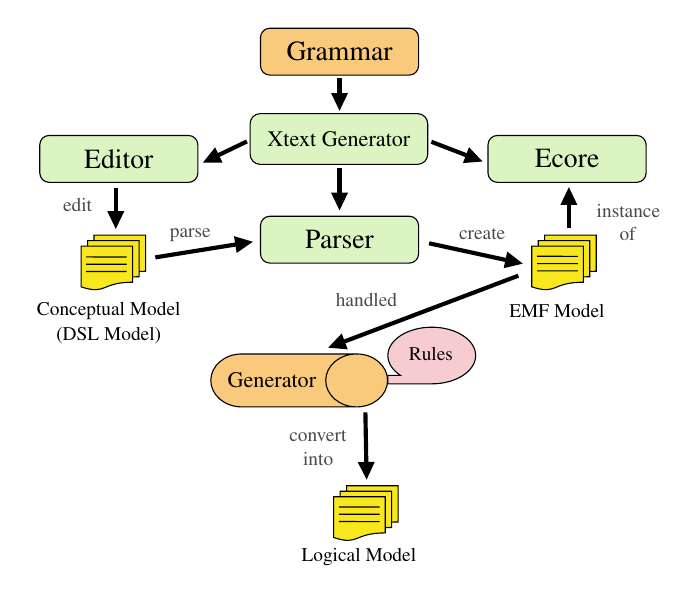
\begin{tikzpicture}[x=0.55pt,y=0.55pt,yscale=-1,xscale=1]
%uncomment if require: \path (0,465); %set diagram left start at 0, and has height of 465

%Rounded Rect [id:dp8080613887465731] 
\draw  [fill={rgb, 255:red, 245; green, 166; blue, 35 }  ,fill opacity=0.6 ] (166.24,24.37) .. controls (166.24,20.97) and (169,18.21) .. (172.4,18.21) -- (263.96,18.21) .. controls (267.36,18.21) and (270.11,20.97) .. (270.11,24.37) -- (270.11,42.84) .. controls (270.11,46.24) and (267.36,49) .. (263.96,49) -- (172.4,49) .. controls (169,49) and (166.24,46.24) .. (166.24,42.84) -- cycle ;
%Rounded Rect [id:dp23877247410758984] 
\draw  [fill={rgb, 255:red, 184; green, 233; blue, 134 }  ,fill opacity=0.5 ] (21.24,94.82) .. controls (21.24,91.42) and (24,88.66) .. (27.4,88.66) -- (118.95,88.66) .. controls (122.36,88.66) and (125.11,91.42) .. (125.11,94.82) -- (125.11,113.3) .. controls (125.11,116.7) and (122.36,119.46) .. (118.95,119.46) -- (27.4,119.46) .. controls (24,119.46) and (21.24,116.7) .. (21.24,113.3) -- cycle ;
%Flowchart: Multidocument [id:dp49717070559395604] 
\draw  [fill={rgb, 255:red, 248; green, 231; blue, 28 }  ,fill opacity=1 ] (56.88,154.12) -- (90.75,154.12) -- (90.75,177.89) .. controls (69.58,177.89) and (73.82,186.46) .. (56.88,180.91) -- cycle ; \draw  [fill={rgb, 255:red, 248; green, 231; blue, 28 }  ,fill opacity=1 ] (52.64,157.72) -- (86.52,157.72) -- (86.52,181.49) .. controls (65.35,181.49) and (69.58,190.06) .. (52.64,184.52) -- cycle ; \draw  [fill={rgb, 255:red, 248; green, 231; blue, 28 }  ,fill opacity=1 ] (48.41,161.32) -- (82.28,161.32) -- (82.28,185.09) .. controls (61.11,185.09) and (65.35,193.66) .. (48.41,188.12) -- cycle ;
%Straight Lines [id:da5642847406466045] 
\draw [fill={rgb, 255:red, 248; green, 231; blue, 28 }  ,fill opacity=1 ]   (51.63,168.47) -- (78.34,168.5) ;
%Straight Lines [id:da9779186616916171] 
\draw [fill={rgb, 255:red, 248; green, 231; blue, 28 }  ,fill opacity=1 ]   (51.63,173.26) -- (78.34,173.28) ;
%Straight Lines [id:da8217185402464098] 
\draw [fill={rgb, 255:red, 248; green, 231; blue, 28 }  ,fill opacity=1 ]   (51.63,178.04) -- (78.34,178.06) ;


%Straight Lines [id:da27204357118531197] 
\draw [line width=1.5]    (71.18,123.3) -- (71.18,146.06) ;
\draw [shift={(71.18,150.06)}, rotate = 270] [fill={rgb, 255:red, 0; green, 0; blue, 0 }  ][line width=0.08]  [draw opacity=0] (11.61,-5.58) -- (0,0) -- (11.61,5.58) -- cycle    ;
%Rounded Rect [id:dp014713549076222021] 
\draw  [fill={rgb, 255:red, 184; green, 233; blue, 134 }  ,fill opacity=0.5 ] (159.43,80.98) .. controls (159.43,77.3) and (162.41,74.31) .. (166.09,74.31) -- (269.45,74.31) .. controls (273.13,74.31) and (276.11,77.3) .. (276.11,80.98) -- (276.11,100.98) .. controls (276.11,104.66) and (273.13,107.65) .. (269.45,107.65) -- (166.09,107.65) .. controls (162.41,107.65) and (159.43,104.66) .. (159.43,100.98) -- cycle ;
%Rounded Rect [id:dp8159423215616721] 
\draw  [fill={rgb, 255:red, 184; green, 233; blue, 134 }  ,fill opacity=0.5 ] (315.72,94.82) .. controls (315.72,91.42) and (318.48,88.66) .. (321.88,88.66) -- (413.44,88.66) .. controls (416.84,88.66) and (419.59,91.42) .. (419.59,94.82) -- (419.59,113.3) .. controls (419.59,116.7) and (416.84,119.46) .. (413.44,119.46) -- (321.88,119.46) .. controls (318.48,119.46) and (315.72,116.7) .. (315.72,113.3) -- cycle ;
%Flowchart: Multidocument [id:dp814245162277164] 
\draw  [fill={rgb, 255:red, 248; green, 231; blue, 28 }  ,fill opacity=1 ] (352.96,154.12) -- (386.83,154.12) -- (386.83,177.89) .. controls (365.66,177.89) and (369.89,186.46) .. (352.96,180.91) -- cycle ; \draw  [fill={rgb, 255:red, 248; green, 231; blue, 28 }  ,fill opacity=1 ] (348.72,157.72) -- (382.6,157.72) -- (382.6,181.49) .. controls (361.43,181.49) and (365.66,190.06) .. (348.72,184.52) -- cycle ; \draw  [fill={rgb, 255:red, 248; green, 231; blue, 28 }  ,fill opacity=1 ] (344.49,161.32) -- (378.36,161.32) -- (378.36,185.09) .. controls (357.19,185.09) and (361.43,193.66) .. (344.49,188.12) -- cycle ;
%Straight Lines [id:da659202853659377] 
\draw [fill={rgb, 255:red, 248; green, 231; blue, 28 }  ,fill opacity=1 ]   (347.97,168.04) -- (374.69,168.06) ;
%Straight Lines [id:da8271632436642871] 
\draw [fill={rgb, 255:red, 248; green, 231; blue, 28 }  ,fill opacity=1 ]   (347.97,172.82) -- (374.69,172.85) ;
%Straight Lines [id:da22701123408508272] 
\draw [fill={rgb, 255:red, 248; green, 231; blue, 28 }  ,fill opacity=1 ]   (347.97,177.61) -- (374.69,177.63) ;


%Straight Lines [id:da6612735011438882] 
\draw [line width=1.5]    (368.86,126.65) -- (368.86,149.4) ;
\draw [shift={(368.86,122.65)}, rotate = 90] [fill={rgb, 255:red, 0; green, 0; blue, 0 }  ][line width=0.08]  [draw opacity=0] (11.61,-5.58) -- (0,0) -- (11.61,5.58) -- cycle    ;
%Rounded Rect [id:dp9641259565957541] 
\draw  [fill={rgb, 255:red, 184; green, 233; blue, 134 }  ,fill opacity=0.5 ] (166.24,147.89) .. controls (166.24,144.48) and (169,141.73) .. (172.4,141.73) -- (263.96,141.73) .. controls (267.36,141.73) and (270.11,144.48) .. (270.11,147.89) -- (270.11,166.36) .. controls (270.11,169.76) and (267.36,172.52) .. (263.96,172.52) -- (172.4,172.52) .. controls (169,172.52) and (166.24,169.76) .. (166.24,166.36) -- cycle ;
%Straight Lines [id:da4555835119587406] 
\draw [line width=1.5]    (218.18,50.89) -- (218.18,68.42) ;
\draw [shift={(218.18,72.42)}, rotate = 270] [fill={rgb, 255:red, 0; green, 0; blue, 0 }  ][line width=0.08]  [draw opacity=0] (11.61,-5.58) -- (0,0) -- (11.61,5.58) -- cycle    ;
%Straight Lines [id:da2586670416419199] 
\draw [line width=1.5]    (218.18,109.78) -- (218.18,133.88) ;
\draw [shift={(218.18,137.88)}, rotate = 270] [fill={rgb, 255:red, 0; green, 0; blue, 0 }  ][line width=0.08]  [draw opacity=0] (11.61,-5.58) -- (0,0) -- (11.61,5.58) -- cycle    ;
%Straight Lines [id:da2552674310073062] 
\draw [line width=1.5]    (157.32,92.59) -- (132.04,104.77) ;
\draw [shift={(128.43,106.51)}, rotate = 334.28] [fill={rgb, 255:red, 0; green, 0; blue, 0 }  ][line width=0.08]  [draw opacity=0] (11.61,-5.58) -- (0,0) -- (11.61,5.58) -- cycle    ;
%Straight Lines [id:da29550662771480396] 
\draw [line width=1.5]    (308.34,104.31) -- (278.52,92.81) ;
\draw [shift={(312.07,105.76)}, rotate = 201.11] [fill={rgb, 255:red, 0; green, 0; blue, 0 }  ][line width=0.08]  [draw opacity=0] (11.61,-5.58) -- (0,0) -- (11.61,5.58) -- cycle    ;
%Straight Lines [id:da3280771928101003] 
\draw [line width=1.5]    (97.15,168.77) -- (157.22,159.13) ;
\draw [shift={(161.17,158.5)}, rotate = 530.89] [fill={rgb, 255:red, 0; green, 0; blue, 0 }  ][line width=0.08]  [draw opacity=0] (11.61,-5.58) -- (0,0) -- (11.61,5.58) -- cycle    ;
%Straight Lines [id:da9478402467031726] 
\draw [line width=1.5]    (277.03,159.51) -- (334.63,172.02) ;
\draw [shift={(338.54,172.87)}, rotate = 192.26] [fill={rgb, 255:red, 0; green, 0; blue, 0 }  ][line width=0.08]  [draw opacity=0] (11.61,-5.58) -- (0,0) -- (11.61,5.58) -- cycle    ;
%Flowchart: Direct Access Storage [id:dp7657317583515377] 
\draw  [fill={rgb, 255:red, 245; green, 166; blue, 35 }  ,fill opacity=0.6 ] (229.43,266.99) -- (153.92,266.99) .. controls (142.69,266.99) and (133.59,259.2) .. (133.59,249.6) .. controls (133.59,240) and (142.69,232.21) .. (153.92,232.21) -- (229.43,232.21)(249.75,249.6) .. controls (249.75,259.2) and (240.65,266.99) .. (229.43,266.99) .. controls (218.2,266.99) and (209.1,259.2) .. (209.1,249.6) .. controls (209.1,240) and (218.2,232.21) .. (229.43,232.21) .. controls (240.65,232.21) and (249.75,240) .. (249.75,249.6) ;
%Straight Lines [id:da100480350897858] 
\draw [line width=1.5]    (335.65,180.79) -- (214.46,226.67) ;
\draw [shift={(210.72,228.08)}, rotate = 339.27] [fill={rgb, 255:red, 0; green, 0; blue, 0 }  ][line width=0.08]  [draw opacity=0] (11.61,-5.58) -- (0,0) -- (11.61,5.58) -- cycle    ;
%Flowchart: Multidocument [id:dp5253239734010293] 
\draw  [fill={rgb, 255:red, 248; green, 231; blue, 28 }  ,fill opacity=1 ] (222.79,318.82) -- (256.67,318.82) -- (256.67,342.59) .. controls (235.5,342.59) and (239.73,351.16) .. (222.79,345.61) -- cycle ; \draw  [fill={rgb, 255:red, 248; green, 231; blue, 28 }  ,fill opacity=1 ] (218.56,322.42) -- (252.44,322.42) -- (252.44,346.19) .. controls (231.26,346.19) and (235.5,354.76) .. (218.56,349.21) -- cycle ; \draw  [fill={rgb, 255:red, 248; green, 231; blue, 28 }  ,fill opacity=1 ] (214.32,326.02) -- (248.2,326.02) -- (248.2,349.79) .. controls (227.03,349.79) and (231.26,358.36) .. (214.32,352.81) -- cycle ;
%Straight Lines [id:da29635223798470123] 
\draw [fill={rgb, 255:red, 248; green, 231; blue, 28 }  ,fill opacity=1 ]   (217.81,332.74) -- (244.53,332.76) ;
%Straight Lines [id:da45709195099870326] 
\draw [fill={rgb, 255:red, 248; green, 231; blue, 28 }  ,fill opacity=1 ]   (217.81,337.52) -- (244.53,337.54) ;
%Straight Lines [id:da9397926099052756] 
\draw [fill={rgb, 255:red, 248; green, 231; blue, 28 }  ,fill opacity=1 ]   (217.81,342.31) -- (244.53,342.33) ;


%Straight Lines [id:da10826901476686546] 
\draw [line width=1.5]    (235.16,270.55) -- (235.89,310.78) ;
\draw [shift={(235.96,314.78)}, rotate = 268.97] [fill={rgb, 255:red, 0; green, 0; blue, 0 }  ][line width=0.08]  [draw opacity=0] (11.61,-5.58) -- (0,0) -- (11.61,5.58) -- cycle    ;
%Flowchart: Sequential Access Storage [id:dp3007368871754543] 
\draw  [fill={rgb, 255:red, 208; green, 2; blue, 27 }  ,fill opacity=0.2 ] (307.6,233.24) .. controls (307.6,222.96) and (294.69,214.63) .. (278.76,214.63) .. controls (262.84,214.63) and (249.93,222.96) .. (249.93,233.24) .. controls (249.93,238.31) and (253.07,242.9) .. (258.17,246.26) -- (249.93,246.26) -- (249.93,251.84) -- (278.76,251.84) .. controls (294.69,251.84) and (307.6,243.51) .. (307.6,233.24) -- cycle ;

% Text Node
\draw (73.18,104.06) node   [align=left] {Editor};
% Text Node
\draw (367.66,104.06) node   [align=left] {Ecore};
% Text Node
\draw (218.18,157.12) node   [align=left] {Parser};
% Text Node
\draw (218.18,33.6) node  [font=\normalsize] [align=left] {Grammar};
% Text Node
\draw (66.54,203.99) node   [align=left] {{\scriptsize Conceptual Model}};
% Text Node
\draw (361.03,203.99) node   [align=left] {{\scriptsize EMF Model}};
% Text Node
\draw (173.76,249.14) node  [font=\footnotesize] [align=left] {\begin{minipage}[lt]{39.427624pt}\setlength\topsep{0pt}
\begin{center}
Generator
\end{center}

\end{minipage}};
% Text Node
\draw (230.86,365.69) node   [align=left] {{\scriptsize Logical Model}};
% Text Node
\draw (278.24,232.37) node  [font=\scriptsize] [align=left] {\begin{minipage}[lt]{20.957804000000003pt}\setlength\topsep{0pt}
\begin{center}
Rules
\end{center}

\end{minipage}};
% Text Node
\draw (34.8,128.16) node [anchor=north west][inner sep=0.75pt]  [font=\scriptsize,color={rgb, 255:red, 74; green, 74; blue, 74 }  ,opacity=1 ] [align=left] {edit};
% Text Node
\draw (105,148.18) node [anchor=north west][inner sep=0.75pt]  [font=\scriptsize,color={rgb, 255:red, 74; green, 74; blue, 74 }  ,opacity=1 ] [align=left] {parse};
% Text Node
\draw (295,148.18) node [anchor=north west][inner sep=0.75pt]  [font=\scriptsize,color={rgb, 255:red, 74; green, 74; blue, 74 }  ,opacity=1 ] [align=left] {create};
% Text Node
\draw (385.4,132.21) node [anchor=north west][inner sep=0.75pt]  [font=\scriptsize,color={rgb, 255:red, 74; green, 74; blue, 74 }  ,opacity=1 ] [align=left] {instance};
% Text Node
\draw (214,190.69) node [anchor=north west][inner sep=0.75pt]  [font=\scriptsize,color={rgb, 255:red, 74; green, 74; blue, 74 }  ,opacity=1 ] [align=left] {handled};
% Text Node
\draw (183.5,280.8) node [anchor=north west][inner sep=0.75pt]  [font=\scriptsize,color={rgb, 255:red, 74; green, 74; blue, 74 }  ,opacity=1 ] [align=left] {convert};
% Text Node
\draw (400.4,147.21) node [anchor=north west][inner sep=0.75pt]  [font=\scriptsize,color={rgb, 255:red, 74; green, 74; blue, 74 }  ,opacity=1 ] [align=left] {of};
% Text Node
\draw (217.77,90.98) node  [font=\footnotesize] [align=left] {Xtext Generator};
% Text Node
\draw (192.5,294.8) node [anchor=north west][inner sep=0.75pt]  [font=\scriptsize,color={rgb, 255:red, 74; green, 74; blue, 74 }  ,opacity=1 ] [align=left] {into};
% Text Node
\draw (66.54,219.99) node   [align=left] {{\scriptsize (DSL Model)}};


\end{tikzpicture}

%     \caption{Xtext architecture.}
%     \label{fig:arqXtext}
% \end{figure}

%#################################################################
\subsection{The Language} \label{sec:EspecDSL}
%#################################################################

\definecolor{javared}{rgb}{0.6,0,0} % for strings
\definecolor{javagreen}{rgb}{0.25,0.5,0.35} % comments
\definecolor{javapurple}{rgb}{0.5,0,0.35} % keywords
\definecolor{javadocblue}{rgb}{0.25,0.35,0.75} % javadoc
\definecolor{verde}{rgb}{0.25,0.5,0.35}
\definecolor{jpurple}{rgb}{0.5,0,0.35}
\definecolor{darkgreen}{rgb}{0.0, 0.2, 0.13}


\lstdefinelanguage{Xtext}{
  sensitive = true,
  keywords={},
  keywords=[2]{ERModel, Domain, Attribute, Entity, Relation, RelationSide, DataType, CardinalityType},
  keywords=[3]{grammar, with, generate, Terminals, enum},
  otherkeywords={*, ?, +, *=, ?=, +=, |},
  keywordstyle=\color{black}\bfseries,
  keywordstyle=[2]\color{javadocblue}\bfseries,
  keywordstyle=[3]\color{javapurple}\bfseries,% for example
%   backgroundcolor=\color{cyan!10},
%   numbers=left,
%   stepnumber=1,
  numbersep=8pt,
  showstringspaces=false,
  breaklines=true,
  frame=top,
  comment=[l]{//},
  morecomment=[s]{/*}{*/},
  commentstyle=\color{black}\ttfamily, 
%   \ttfamily \bfseries
  stringstyle=\color{javared},
  morestring=[b]',
  morestring=[b]"
  }
  
  \lstdefinelanguage{Xtext2}{
  sensitive = true,
  keywords={},
  keywords=[2]{ERModel, Domain, Attribute, Entity, Relation, RelationSide, DataType, CardinalityType},
  keywords=[3]{grammar, with, generate, Terminals, enum},
  otherkeywords={*, ?, +, *=, ?=, +=, |},
  keywordstyle=\color{black}\bfseries,
  keywordstyle=[2]\color{javadocblue}\bfseries,
  keywordstyle=[3]\color{javapurple}\bfseries,% for example
  backgroundcolor=\color{cyan!10},
  numbers=left,
  stepnumber=1,
  numbersep=8pt,
  showstringspaces=false,
  breaklines=true,
  frame=top,
  comment=[l]{//},
  morecomment=[s]{/*}{*/},
  commentstyle=\color{black}\ttfamily,
  stringstyle=\color{javared}\ttfamily,
  morestring=[b]',
  morestring=[b]"
  }
  
  \lstdefinelanguage{ERDSL}{
  sensitive = true,
  keywords={},
  keywords=[2]{Domain, Entities, Relationships, isIdentifier, isRelatedWith, isA, zero, one, many},
  keywords=[3]{int, money, string, datetime, file},
  otherkeywords={*, ?, +, *=, ?=, +=, |},
  keywordstyle=\color{black}\bfseries,
  keywordstyle=[2]\color{javapurple}\bfseries,
  keywordstyle=[3]\color{javadocblue}\bfseries,% for example
%   backgroundcolor=\color{cyan!10},
%   numbers=left,
%   stepnumber=1,
  captionpos=t,
  numbersep=8pt,
  showstringspaces=false,
  breaklines=true,
  frame=top,
  comment=[l]{//},
  morecomment=[s]{/*}{*/},
  commentstyle=\color{black}\ttfamily,
  stringstyle=\color{javared}\ttfamily,
  morestring=[b]',
  morestring=[b]"
  }
  
  \lstdefinelanguage{BNF}{
  sensitive = true,
  keywords={},
  keywords=[2]{},
  otherkeywords={::= , |, <, >},
  keywordstyle=\color{javapurple}\bfseries,
  keywordstyle=[2]\color{javapurple}\bfseries,
  keywordstyle=[3]\color{javadocblue}\bfseries,% for example
%   backgroundcolor=\color{cyan!10},
%   numbers=left,
%   stepnumber=1,
  captionpos=t,
  numbersep=8pt,
  showstringspaces=false,
  breaklines=true,
  frame=top,
  comment=[l]{//},
  morecomment=[s]{/*}{*/},
  commentstyle=\color{darkgreen}\ttfamily,
  stringstyle=\color{javared}\ttfamily,
  morestring=[b]',
  morestring=[b]"
  }
  
  
  
  

In the current phase of the work, the language at the conceptual level is not fully finalized.
There are topics related to scope validation, as in the case of the treatment of unwanted cross-references and other restrictions inherent to the ER model that must be analyzed and then implemented.
The definition of the created DSL is displayed in Figure \ref{fig:DSLvsFinal}.

\lstset{basicstyle=\tiny}
\begin{figure}[!htb]
    \centering
    \begin{scriptsize}
    \begin{lstlisting}[language = Xtext , frame = trbl]
grammar org.xtext.unipampa.lesse.ertext.ERtext 
with org.eclipse.xtext.common.Terminals
generate ERtext "xtext.org/unipampa/lesse/ertext"
ERModel:
	domain=Domain ';'
	('Entities' '{') entities+=Entity+ ('}' ';')
	('Relationships' '{')relations+=Relation*('}'';');
Domain:
	'Domain' name=ID;
Attribute:
        name=ID type=DataType (isKey?='isIdentifier')?;
Entity:
	name=ID ('is' is+=[Entity])*
	('{' attributes+=Attribute 
	(',' attributes+=Attribute)* '}')?;
Relation:
	(name=ID)? ('[' leftEnding=RelationSide 
	'relates' 
	rightEnding=RelationSide ']') 
	('{' attributes+=Attribute 
	(',' attributes+=Attribute)* '}')*;
RelationSide:
	cardinality=('(0:1)' | '(1:1)' | '(0:N)' | '(1:N)') 
	target=[Entity] | target=[Relation];
enum DataType:
        INT='int'           | DOUBLE='double'       | 
        MONEY='money'       | STRING='string'       |
        BOOLEAN='boolean'   | DATETIME='datetime'   |
        BLOB='file';
    \end{lstlisting}
    \end{scriptsize}
    \caption{Grammar definition of the DSL.}
    \label{fig:DSLvsFinal}
\end{figure}

% The \texttt{grammar} command specifies the DSL name, while the \texttt{with} statement declares an inheritance from another language.
% In the case of the proposed grammar, a standard Xtext grammar, called \texttt{Terminals}, will be used, which provides some predefined rules, \textit{e.g.} the rule \texttt{ID} for identifiers or \texttt{INT} for integers.
% The \texttt{generate} command is the statement that produces the language's AST.

% The first rule, called the input rule, defines what the general language structure looks like.
% Words and symbols in double or single quotes indicate reserved words.
% For example, the object \texttt{Entities} must be preceded by ``\texttt {Entities\{}''.
% This object represents a kind of a container indicated through the assignment operator \texttt{+=}.
% It is an object that can contain other objects, in this case one or more instances of \texttt{Entity}.
% It is established that each DSL file must also be composed of a \texttt{Domain} and zero or more \texttt{Relation}.

% The multiplicity is indicated by \texttt{*} (zero or many), \texttt{+} (one or many) or \texttt{?} (zero or one).
% By not placing any of these operators, then one implicitly is expected to occur.
% Regarding assignments, when only one \texttt{=} is specified, it means that the object on the left side expects only one record.
% Therefore, for \texttt{+=} then zero, one or more occurrences are expected.

% The \texttt{Domain} object is preceded by a reserved word with the same name, followed by an identifier.
% The entity is defined by the \texttt{Entity} statement together with identifier name for this object.
% Defining an inheritance is optional using the reserved word \texttt{is}.
% After defining the name, a body of keys opens in which the entity attributes are specified.
% An entity must contain at least one attribute, but it does not need to be an identifier because of the possible existence of weak entities.

% The compound rules are only performed due to the possibility of grouping expressions using parentheses, in addition to the possibility of using other rules through cross-references.
% The brackets between the \texttt{Entity} rule are used to indicate that you want to use only the \texttt{name} attribute that identifies the object.
% Entity attributes are defined by a name, inheriting the \texttt{ID} rule from \texttt{Terminals}, and optional attributes \textit{e.g.} \texttt{isIdentifier} to symbolize primary keys.

% The relationship is defined, already within the body of the \texttt{Relationships} block, with an optional declaration of its identification.
% Then, brackets are opened and two elements must be specified \texttt{RelationSide} as a reference to the attributes \texttt{leftEnding} and \texttt{rightEnding}.
% These attributes represent the sides of a relationship.
% These objects must be separated by the expression \texttt{relates}.
% The sides of the relation are defined in the rule \textit{RelationSide}, composed of two attributes.
% The \texttt{cardinality} attribute is mandatory and uses numerals \texttt{(0:1), (1:1), (0:N), (1:N)}.
% The \texttt{target} attribute is likewise mandatory, accepting a cross-reference to a \texttt{Entity} or \texttt{Relation}.
% In the case of a \texttt{target} referencing a \texttt{Relation}, then a ternary relationship is highlighted.

% The attribute types are contained in an enumerated list called \texttt{DataType}, on the left side is the representation in the model \textit{Ecore}.
% On the right side is the reserved word that is used in the language.
% The conditional symbol \texttt{|} means the logical operator \textit{OR} and serves to separate each definition \texttt{<key> = <value>} as an option within the list.

% %#########################################################
% \subsection{ERtext Operation}
% %#########################################################

% With the development of the DSL, the stabled version of the grammar resulted from the merger between the two previously defined versions  and evaluated with the execution of a focus group.
% % \cite{krueger:2002}
% % The main changes were the modifications of the reserved words \texttt{isA} and \texttt{isRelatedWith} by \texttt{is} and \texttt{relates}, respectively, in addition to the adoption of the convention \texttt{(0:1) (1:1) (0:N) (1:N)} for the cardinalities.

% % A \autoref{fig:ERTextUso} apresenta a ferramenta em funcionamento, onde é possível ser feita a criação de arquivos de modelagem utilizando a DSL. 
% % In this example, 7 entities and 6 relationships are modeled, including a self-relationship and a ternary relationship.
% In the instruments\footnote{Supplemental Materials for the Experiment: Available at Zenodo: \url{https://doi.org/10.5281/zenodo.4056791}} problems used to the experiment, 7$\sim$9 entities were modeled, with binary, ternary and recursive relationships as well as different kind of attributes add up to between 40 and 47 items.

% % https://doi.org/10.5281/zenodo.4056791
% % https://doi.org/10.5281/zenodo.4056791

% Modeling in the tool gains real-time validation, syntax highlighting that indicates syntax errors in editing time, code completion and hovering, a feature that displays information about an item in mouse over events.

% % It is known that the definition of data types is not foreseen in the classic conceptual model but, due to issues related to the future intention to perform the generation of SQL statements, it was decided to maintain this design decision.

% % \begin{figure}[!htb]
% %     \centering
% %     \caption{Fragmento da solução sendo utilizada.}
% %     \label{fig:ERTextUso}
% %     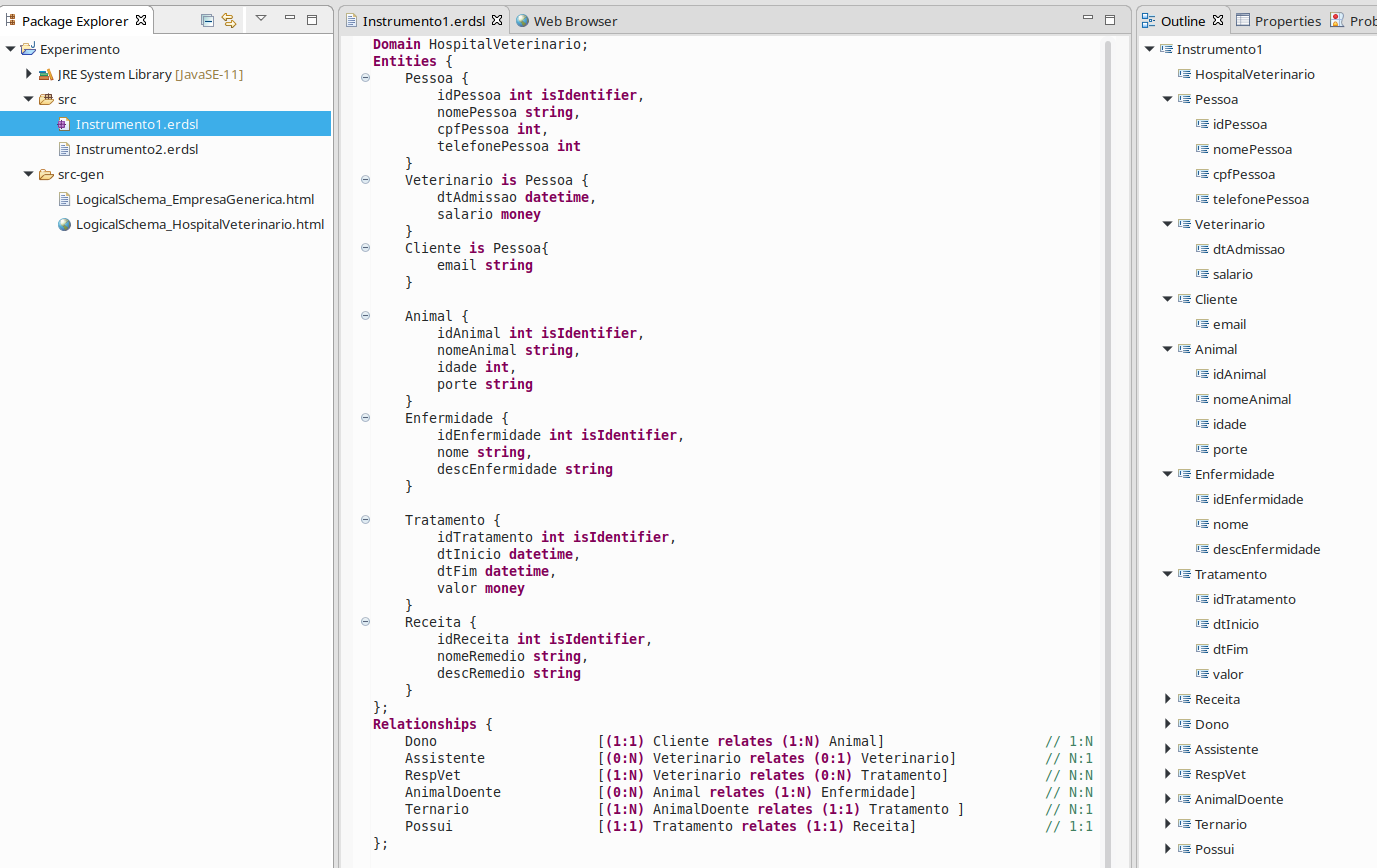
\includegraphics[width=0.4\textwidth]{images/ERTextUso.png}
% % \end{figure}

% The function for mapping and generating the logical model is performed automatically every time a model is saved.
% The environment generates \texttt{.html} files in a specific directory structure.
% % Files with this format were generated for a better view from the text markings.
% % These markings can be rendered by any browser, or even within the modeling tool, increasing the power of understanding and usefulness by the user.

% % The logical model derived by the generator that maps the conceptual model is presented in \autoref{fig:modeloLogico}.
% % \begin{figure}[!htb]
% %     \centering
% %     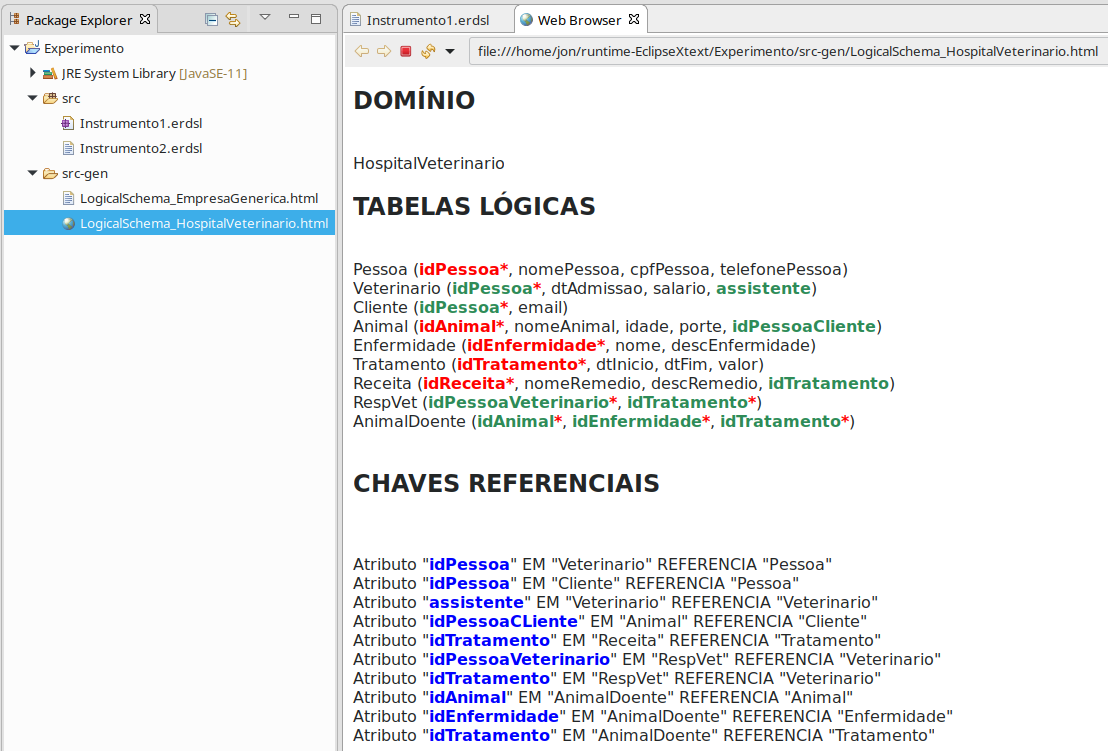
\includegraphics[width=0.9\columnwidth]{images/ModeloLogico.png}
% %     \caption{Example of generated logical model.}
% %     \label{fig:modeloLogico}
% % \end{figure}

% Based on these transformation assumptions, the original model results in a new model composed of entities, and also already having their inferred reference integrity, \textit{i.e.} the records pointing to other records are already established.
% To apply the mapping between the models, we adopted the assumptions proposed by Heuser \cite{Heuser:2009}.
% % alternatives between the models.
% % the ones marked are those that were implemented up to the time of delivery of this study.

% % \begin{figure}[!htb]
% %     \centering
% %     \caption{Assumptions adopted for the transformation between models.}
% %     \label{fig:Premissas}
% %     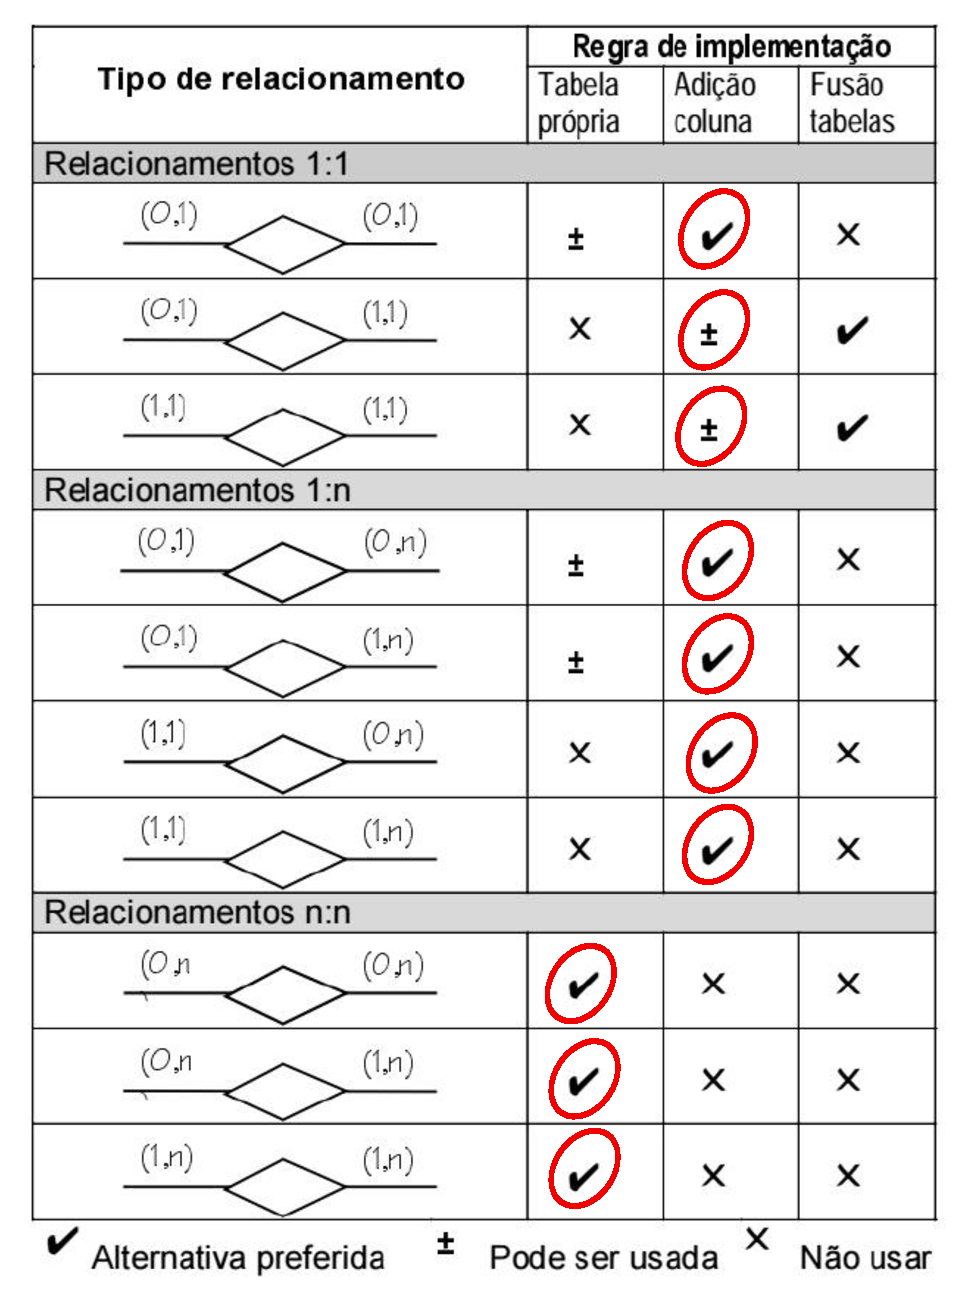
\includegraphics[width=0.35\textwidth]{images/TabelaMapeamentoRelacionamentos.eps}
% % \end{figure}

% Regarding the generalization concepts, we also assume another assumption from Heuser \cite{Heuser:2009}, which maps for the transformation between models (from conceptual to logical). Two alternatives that can be derived:
% % 1) The first one recommends the use of a single table for the entire hierarchy of entities, \textit{i.e.} it recommends merging the tables; a 2) The second one recommends the use of a table by modeled entity, as long as respecting referential integrity, \textit{i.e.} the primary keys of the child entities must necessarily point to the primary key of the parent entity, creating a foreign keys references. Then, we chose the second alternative for such a design decision.

% The generator of the logical model was developed with GPL Xtend, and carry out the transformation from conceptual to logical models.
% % The generator of the logical model was developed with GPL Xtend, and currently has about four hundred lines of code to carry out the transformation from conceptual to logical models.


%#######################################################
%#######################################################
\section{\uppercase{Empirical Evaluation}} 
\label{sec:evaluation}
%#######################################################%#######################################################

% \begin{figure}[!htb]
%     \centering
%     

\tikzset{every picture/.style={line width=0.75pt}} %set default line width to 0.75pt        

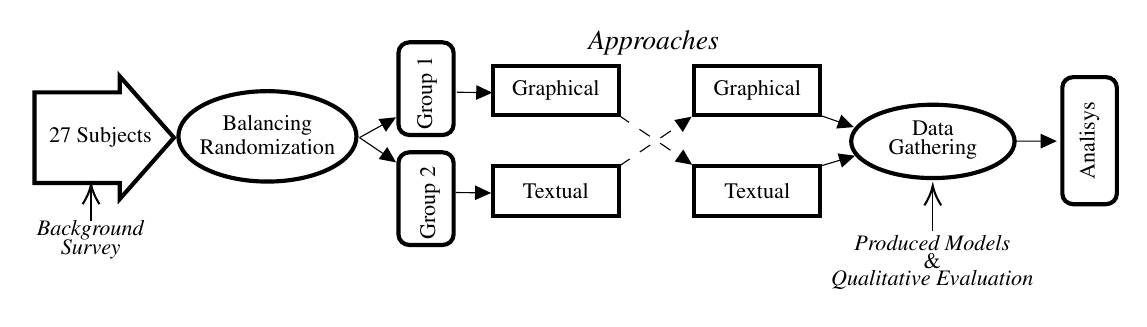
\begin{tikzpicture}[x=0.65pt,y=0.62pt,yscale=-1,xscale=1]
%uncomment if require: \path (0,193); %set diagram left start at 0, and has height of 193


%Shape: Ellipse [id:dp633810982278807] 
\draw  [line width=1.5]  (104.59,88.03) .. controls (104.59,73.48) and (126.76,61.68) .. (154.09,61.68) .. controls (181.43,61.68) and (203.59,73.48) .. (203.59,88.03) .. controls (203.59,102.57) and (181.43,114.37) .. (154.09,114.37) .. controls (126.76,114.37) and (104.59,102.57) .. (104.59,88.03) -- cycle ;


%Shape: Ellipse [id:dp7904221795411808] 
\draw  [line width=1.5]  (478.63,90.96) .. controls (478.63,79.15) and (498.97,69.58) .. (524.05,69.58) .. controls (549.13,69.58) and (569.46,79.15) .. (569.46,90.96) .. controls (569.46,102.76) and (549.13,112.33) .. (524.05,112.33) .. controls (498.97,112.33) and (478.63,102.76) .. (478.63,90.96) -- cycle ;

%Rounded Rect [id:dp5302697683495847] 
\draw  [line width=1.5]  (226.94,103.44) .. controls (226.94,100.05) and (229.69,97.31) .. (233.07,97.31) -- (251.46,97.31) .. controls (254.85,97.31) and (257.59,100.05) .. (257.59,103.44) -- (257.59,145.19) .. controls (257.59,148.58) and (254.85,151.33) .. (251.46,151.33) -- (233.07,151.33) .. controls (229.69,151.33) and (226.94,148.58) .. (226.94,145.19) -- cycle ;
%Rounded Rect [id:dp9616486966995694] 
\draw  [line width=1.5]  (226.94,39.34) .. controls (226.94,35.96) and (229.69,33.21) .. (233.07,33.21) -- (251.46,33.21) .. controls (254.85,33.21) and (257.59,35.96) .. (257.59,39.34) -- (257.59,81.1) .. controls (257.59,84.49) and (254.85,87.23) .. (251.46,87.23) -- (233.07,87.23) .. controls (229.69,87.23) and (226.94,84.49) .. (226.94,81.1) -- cycle ;
%Shape: Rectangle [id:dp03801896284105699] 
\draw  [line width=1.5]  (279.43,46.83) -- (349.43,46.83) -- (349.43,75.81) -- (279.43,75.81) -- cycle ;
%Straight Lines [id:da1799424135415575] 
\draw    (205.3,88.75) -- (223,78.43) ;
\draw [shift={(225.59,76.91)}, rotate = 509.75] [fill={rgb, 255:red, 0; green, 0; blue, 0 }  ][line width=0.08]  [draw opacity=0] (8.93,-4.29) -- (0,0) -- (8.93,4.29) -- cycle    ;
%Straight Lines [id:da17029537209985257] 
\draw    (205.3,88.75) -- (223.15,101.44) ;
\draw [shift={(225.59,103.18)}, rotate = 215.43] [fill={rgb, 255:red, 0; green, 0; blue, 0 }  ][line width=0.08]  [draw opacity=0] (8.93,-4.29) -- (0,0) -- (8.93,4.29) -- cycle    ;
%Straight Lines [id:da39402523544663426] 
\draw  [dash pattern={on 4.5pt off 4.5pt}]  (349.71,105.32) -- (387.49,78.28) ;
\draw [shift={(389.93,76.54)}, rotate = 504.41] [fill={rgb, 255:red, 0; green, 0; blue, 0 }  ][line width=0.08]  [draw opacity=0] (8.93,-4.29) -- (0,0) -- (8.93,4.29) -- cycle    ;
%Straight Lines [id:da7992081880522388] 
\draw  [dash pattern={on 4.5pt off 4.5pt}]  (349.43,75.81) -- (387.76,102.86) ;
\draw [shift={(390.21,104.59)}, rotate = 215.21] [fill={rgb, 255:red, 0; green, 0; blue, 0 }  ][line width=0.08]  [draw opacity=0] (8.93,-4.29) -- (0,0) -- (8.93,4.29) -- cycle    ;
%Right Arrow [id:dp6900414397065515] 
\draw  [line width=1.5]  (24.59,62.36) -- (72.02,62.36) -- (72.02,53.02) -- (102.12,88.77) -- (72.02,124.52) -- (72.02,115.17) -- (24.59,115.17) -- cycle ;
%Shape: Rectangle [id:dp003852149638719382] 
\draw  [line width=1.5]  (391.43,46.83) -- (461.43,46.83) -- (461.43,75.81) -- (391.43,75.81) -- cycle ;
%Shape: Rectangle [id:dp0126542660109914] 
\draw  [line width=1.5]  (391.43,105.34) -- (461.43,105.34) -- (461.43,134.33) -- (391.43,134.33) -- cycle ;
%Shape: Rectangle [id:dp4954877903085966] 
\draw  [line width=1.5]  (279.43,105.34) -- (349.43,105.34) -- (349.43,134.33) -- (279.43,134.33) -- cycle ;
%Straight Lines [id:da3442884963113835] 
\draw    (461.43,75.81) -- (477.28,81.6) ;
\draw [shift={(480.1,82.62)}, rotate = 200.04] [fill={rgb, 255:red, 0; green, 0; blue, 0 }  ][line width=0.08]  [draw opacity=0] (8.93,-4.29) -- (0,0) -- (8.93,4.29) -- cycle    ;
%Straight Lines [id:da6883068419855551] 
\draw    (461.43,105.34) -- (477.9,100.19) ;
\draw [shift={(480.77,99.29)}, rotate = 522.63] [fill={rgb, 255:red, 0; green, 0; blue, 0 }  ][line width=0.08]  [draw opacity=0] (8.93,-4.29) -- (0,0) -- (8.93,4.29) -- cycle    ;
%Rounded Rect [id:dp5928061300931144] 
\draw  [line width=1.5]  (596,59.56) .. controls (596,56.21) and (598.71,53.5) .. (602.06,53.5) -- (620.24,53.5) .. controls (623.59,53.5) and (626.3,56.21) .. (626.3,59.56) -- (626.3,121.49) .. controls (626.3,124.84) and (623.59,127.55) .. (620.24,127.55) -- (602.06,127.55) .. controls (598.71,127.55) and (596,124.84) .. (596,121.49) -- cycle ;

%Straight Lines [id:da6932528701926595] 
\draw    (569.46,90.81) -- (589.92,90.8) ;
\draw [shift={(592.92,90.8)}, rotate = 539.96] [fill={rgb, 255:red, 0; green, 0; blue, 0 }  ][line width=0.08]  [draw opacity=0] (8.93,-4.29) -- (0,0) -- (8.93,4.29) -- cycle    ;
%Straight Lines [id:da7950818392289087] 
\draw    (56.04,137.1) -- (56.04,118.09) ;
\draw [shift={(56.04,116.09)}, rotate = 450] [color={rgb, 255:red, 0; green, 0; blue, 0 }  ][line width=0.75]    (10.93,-4.9) .. controls (6.95,-2.3) and (3.31,-0.67) .. (0,0) .. controls (3.31,0.67) and (6.95,2.3) .. (10.93,4.9)   ;
%Straight Lines [id:da5784112946450906] 
\draw    (523.97,143.21) -- (523.97,118.78) ;
\draw [shift={(523.97,116.78)}, rotate = 450] [color={rgb, 255:red, 0; green, 0; blue, 0 }  ][line width=0.75]    (10.93,-4.9) .. controls (6.95,-2.3) and (3.31,-0.67) .. (0,0) .. controls (3.31,0.67) and (6.95,2.3) .. (10.93,4.9)   ;
%Straight Lines [id:da04489153588175898] 
\draw    (259.43,62.29) -- (276.1,62.53) ;
\draw [shift={(279.1,62.58)}, rotate = 180.84] [fill={rgb, 255:red, 0; green, 0; blue, 0 }  ][line width=0.08]  [draw opacity=0] (8.93,-4.29) -- (0,0) -- (8.93,4.29) -- cycle    ;
%Straight Lines [id:da30869554668079413] 
\draw    (258.76,120.74) -- (275.43,120.99) ;
\draw [shift={(278.43,121.03)}, rotate = 180.84] [fill={rgb, 255:red, 0; green, 0; blue, 0 }  ][line width=0.08]  [draw opacity=0] (8.93,-4.29) -- (0,0) -- (8.93,4.29) -- cycle    ;

% Text Node
\draw (314.43,61.32) node  [font=\footnotesize] [align=left] {Graphical};
% Text Node
\draw (611.15,90.53) node  [font=\footnotesize,rotate=-270] [align=left] {Analisys};
% Text Node
\draw (523.67,171.82) node  [font=\footnotesize] [align=left] {\textit{Qualitative Evaluation}};
% Text Node
\draw (523.67,160.67) node  [font=\footnotesize] [align=left] {\&};
% Text Node
\draw (523.67,150.26) node  [font=\footnotesize] [align=left] {\textit{Produced Models}};
% Text Node
\draw (237.48,149.82) node [anchor=north west][inner sep=0.75pt]  [font=\footnotesize,rotate=-270] [align=left] {Group 2};
% Text Node
\draw (426.43,61.32) node  [font=\footnotesize] [align=left] {Graphical};
% Text Node
\draw (314.43,119.83) node  [font=\footnotesize] [align=left] {Textual};
% Text Node
\draw (426.43,119.83) node  [font=\footnotesize] [align=left] {Textual};
% Text Node
\draw (524.05,83.17) node  [font=\footnotesize] [align=left] {Data};
% Text Node
\draw (524.05,95.85) node  [font=\footnotesize] [align=left] {Gathering};
% Text Node
\draw (61.21,88.77) node  [font=\footnotesize] [align=left] {27 Subjects};
% Text Node
\draw (55.78,142.48) node  [font=\footnotesize] [align=left] {\textit{Background}};
% Text Node
\draw (55.78,154.07) node  [font=\footnotesize] [align=left] {\textit{Survey}};
% Text Node
\draw (154.09,81.68) node  [font=\footnotesize] [align=left] {Balancing};
% Text Node
\draw (154.09,94.37) node  [font=\footnotesize] [align=left] {Randomization};
% Text Node
\draw (235.77,85.72) node [anchor=north west][inner sep=0.75pt]  [font=\footnotesize,rotate=-270] [align=left] {Group 1};
% Text Node
\draw (331,25) node [anchor=north west][inner sep=0.75pt]   [align=left] {\textit{Approaches}};


\end{tikzpicture}

%     \caption{Experiment design.}
%     \label{fig:ExperimentDesign}
% \end{figure}

This section exposes the controlled experiment that was performed in order to verify the feasibility of using the textual approach (ERtext) developed in this work in the context of teaching entity-relationship modeling.
% Activities were carried out that involved the execution of modeling practices comparing the results of the proposal of this study with the graphical approach (brModelo), a tool recognized for teaching database in undergraduate courses.
% Quantitative and qualitative analyzes of the results collected from the experiment were carried out using metrics related to effort, 
% %(time spent), 
% precision, recall, F-Measure, as well as qualitative questionnaires to assess items regarding the perceived ease of use and usefulness of both approaches.
% There was a choice of an experimental approach for evaluating the proposal, which was carried out based on the definition of prior planning.
% Hence, 
We followed the guidances and recommendations raised in~\cite{Wohlin:2012}.

%#################################################################
\subsection{Planning}
%#################################################################

The experiment aims to obtain evidence from the comparison of two approaches to the modeling of relational databases, one in a graphical and another in a textual way.
The titled treatments, were:
\begin{inparaenum}[(i)]
\item Control treatment: the brModelo tool, with a graphical approach, and;
\item Experimental treatment: the ERtext tool, with a textual approach.
\end{inparaenum}
The purpose of this experiment is to assess the feasibility of using a textual approach to support the teaching-learning process of conceptual modeling of relational databases.

%#################################################################
%\subsubsection{Research Questions} \label{ssec:questPesq}
%#################################################################

\textbf{Research Questions (RQs)}: For the discussion of the experiment results, we decided to formulate four RQs that were related to the activities performed.

%\begin{description}
%\item 
    \textbf{RQ1.} Which approach requires the most effort spent on average during the modeling activity?
%\item 
    \textbf{RQ2.} What is the quality level of the models produced using the graphical and textual approaches?
%\item 
    \textbf{RQ3.} What is the subjects perception regarding the perceived ease of use (PEOU) and perceived usefulness (PU) of the proposed DSL?
%\item 
    \textbf{RQ4.} What is the subjects assessment in relation to the representation of the ER modeling builders supported in the proposed DSL?
%\end{description}

%#################################################################
%\subsubsection{Context} \label{ssec:contxExp}
%#################################################################

\textbf{Context}: The experiment context is characterized according to four dimensions:
\begin{inparadesc}
    \item \textbf{(i) Process}: An \textit{in-vitro} approach was used, since the tasks were performed in the lab under controlled conditions and without online activities.
    \item \textbf{(ii) Subjects}: Undergrad, master and doctoral students in Computer Science and Software Engineering.
    \item \textbf{(iii) Reality}: The experiment addressed a real problem, that is, the difference in the effort spent of subjects in the conceptual modeling of relational databases, the artifacts quality produced and the subjects perceived usefulness (PU) using both approaches.
    \item \textbf{(iv) Generality:} This evaluation is inserted in a specific context, involving database modeling students. 
    However, the general ideas of this experiment can be replicated in another set of subjects, approaches or DSLs that support database modeling.
\end{inparadesc}

%#################################################################
%\subsubsection{Hypotheses Formulation} \label{ssec:hipExp}
%#################################################################

\textbf{Hypotheses Formulation}: the first two RQs were taken into account. Regarding to \textbf{RQ1.} the average effort spent required using each approach, our scientific hypotheses are as follows:

\textbf{Null hypothesis:} $H_0 : \mu Time_G = \mu Time_T :$ 
There is no difference in average effort spent measure between textual and graphical approaches during conceptual modeling of relational databases.

\textbf{Alternative hypothesis:} $H_{1} : \mu Time_T \neq Time_G :$ There is a significant difference in average effort spent measure between textual and graphical approaches during conceptual modeling of relational databases.

Regarding to \textbf{RQ2.} the modeling effectiveness using each approach, our hypotheses are as follows:

\textbf{Null hypothesis:} $H_0 : \mu Effectiveness_G = \mu 
\\ Effectiveness_T :$ 
There is no difference in effectiveness measure between textual and graphical approaches during conceptual modeling. %of relational databases.

\textbf{Alternative hypothesis:} $H_{1} : \mu Effectiveness_T \neq \mu  Effectiveness_G :$ There is a significant difference in effectiveness measure between textual and graphical approaches during conceptual modeling. %of relational databases.

For the evaluation related to the effort measure, the Shapiro-Wilk normality test 
% \cite{Das:2016} 
and the paired T-test for dependent samples 
% \cite{Xu:2017} 
were used, in which the times collected during the execution of the modeling activities of the experiment were taken into account.
% The Shapiro-Wilk test tests the null hypothesis that a distribution is normal, by calculating the value of $W$, where afterwards it is verified in the test table if the hypothesis is rejected or accepted.
% \footnote{\url{http://www.uel.br/projetos/experimental/pages/arquivos/Probabilidades\_Shapiro.pdf}} 
% The Shapiro-Wilk test calculation is given according to the formula in Equation \ref{eq:Shapiro}:

% \begin{equation}
% \label{eq:Shapiro}
% %\[ 
% W = \frac{\left(\sum_{i=1}^{n} a_ix_{(i)}\right)^2}{\sum_{i=1}^{n}\left(x_i -\overline{x}\right)} 
% %\]
% \end{equation}

% A simplified form of the paired T-test for dependent samples is given according to the formula in Equation \ref{eq:TestT}:

% \begin{equation}
% \label{eq:TestT}
% %\[ 
% t = \frac{m}{s/\sqrt{n}} 
% %\]
% \end{equation}

% In this formula \textit{\textbf{m}} and \textit{\textbf{s}} are the average and standard deviation of the difference (\textbf{\textit{d}}), respectively.
% The \textit{\textbf{n}} corresponds to the size of \textbf{\textbf{d}}, \textit{i.e.} the sample size.
% This hypothesis test is used to compare the means of two related samples, \textit{i.e.}, when there are two values (pair of values) for the same sample.
% However, to compare the averages of the two paired data sets, firstly, the differences among all pairs must be calculated.
% The level of alpha significance ($\alpha$) used was five percent (5\%).
% The Shapiro-Wilk and paired T-test calculations were performed with the support of the R language.
% % \footnote{https://www.rdocumentation.org/packages/stats/versions/3.6.1/topics/shapiro.test}
% % \footnote{https://www.rdocumentation.org/packages/stats/versions/3.6.1/topics/t.test}.

For the effectiveness tests, the same statistical methods were adopted, but instead of using the time metric, another quantity was necessary.
Thus, the \textit{F-Measure} 
%or \textit{F-Score} 
calculations were performed, which is derived from harmonic mean of \textit{Precision} and \textit{Recall} metrics, for each of the models produced in the approaches.
The \textit{F-Measure} \citep{Derczynski:2016} calculation takes into account variables known as \textit{True Positives}, \textit{False Positives} and \textit{False Negatives}.
% \begin{itemize}
%     \item \textbf{\textit{True Positives (TP)}}: Amount of elements correctly modeled using the approach.
%     \item \textbf{\textit{False Positives (FP)}}: Amount of elements incorrectly modeled using the approach. 
%     \item \textbf{\textit{False Negatives (FN)}}: Amount of elements not modeled using the approach.
% \end{itemize}
From the variables identification it is then possible to calculate the \textit{Precision}, \textit{Recall} and \textit{F-Measure} of each model.
% according to the formulas:
% \begin{itemize}
%     \item \textbf{\textit{Precision (P)}}: $\frac{TP}{TP~+~FP}$ 
%     \item \textbf{\textit{Recall (R)}}:$\frac{TP}{TP~+~FN}$ 
%     \item \textbf{\textit{F-Measure (F)}}: $\frac{2~*~(P~*~ R)}{P~+~R}$
% \end{itemize}

%#################################################################
%\subsubsection{Selection of Subjects} %\label{ssec:participExp}
%#################################################################

\textbf{Selection of Subjects}: The subjects were selected by non-probabilistic sampling, indicated for exploratory studies.
This type of sampling is characterized by the deliberate choice of subjects with one or more characteristics that interest to the study object.

In this context, 27 undergrads (Computer Science and Software Engineering) and post-grads (Software Engineering) students from our university participated In this experiment.
Among the subjects there were 14 students enrolled in database course.
After identifying the potential subjects, the execution date of the controlled experiment was defined, which included training in both approaches.
In addition, before the training, subjects would be asked to complete a profile questionnaire for leveling.
From the data extracted of questionnaires, the subjects were randomly distributed into two groups composed of 13 and 14 subjects. 
The reason for that it is because the total number of subjects was odd, and we also tried to maintain a balanced level of skills among the groups.

%#################################################################
%\subsubsection{Experiment Design} \label{ssec:designExp}
%#################################################################

\textbf{Experiment Design}: According to \citet{Wohlin:2012}, a controlled experiment must meet some fundamental concepts:
\begin{inparaenum}[(i)]
\item Standard Design Type: 
There are a few possible types for the standard design in an experiment, and this study adopted One Factor with Two Treatments.
The Factor was the modeling of relational databases, and the Treatments were the two approaches used (graphical and textual).
\item Blocking: 
This item refers to the fact that the subjects of the controlled experiment may have different experience levels in database modeling and design.
As a result, a profile questionnaire was applied to level the subjects.
\item Balancing: 
Subjects were separated into two groups with similar background levels.
In this way, both approaches were carried out by homogeneous groups.
\item Randomization: 
The subjects were randomly allocated to each group and approach.
They performed both treatments, featuring a paired comparison design.
The execution sequence of the treatments for each group was also randomly defined.
\end{inparaenum}

% The \autoref{fig:designExp} displays the evaluation experimental design.
After all the activities performed by the subjects using the treatments, we collect the data results.
This stage consists of the qualitative assessment made by the subjects and the saving of the models produced by the treatments application.
These models serve for a qualitative assessment.
Finally, the analysis stage is performed, where the result data are compiled and analyzed with the aim of drawing conclusions.

% \begin{figure}[!htb]
%     \centering
%     % \include{samples/imgs/DesignExperimento}
%     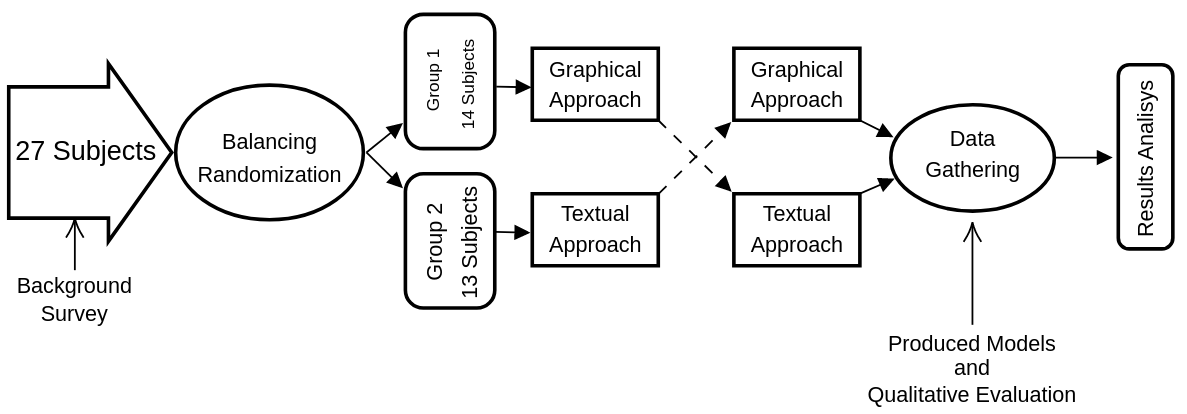
\includegraphics[width=\columnwidth]{images/DesignExperimento.png}
%     \caption{Experiment Design.}
%     \label{fig:designExp}
% \end{figure}

%###########################################################
%\subsubsection{Instrumentation} \label{ssec:instExp}
%###########################################################

\textbf{Instrumentation}: As participation in this experiment was voluntary, a Free, Prior and Informed Consent (FPIC) was prepared %for the subjects 
to record the agreement of all them in carrying out the activities.
Profile questionnaires were created and applied to balance the groups.
Beyond, a glossary was also developed for concepts that were used in the opening presentation of the controlled experiment and during training.
In order to provide support to the evaluation subjects, instruments were provided describing the step by step with use examples of both tools (brModelo and ERtext) used in this experiment.
In addition, training was conducted that included videos with tutorials on how to use the approaches in each tool.
The videos showed how to start modeling, problem examples of the builders foreseen that they would solve and recommendations for saving the artifacts produced.

We elaborated two instruments that contained a problem each, with similar levels of complexity, which should be modeled and also noted the start and end times of the activity.
For further subjects evaluation, we prepared two other instruments.
The first instrument presented 7 quality attributes based on ISO/IEC 25010, %\cite{ISO25010}
a standard for software product quality, and served to evaluate the approaches of the two tools from the point of view of the subjects who performed the ER modeling activities.
The second instrument was used to evaluate the ER modeling builders representation of the textual approach solution evaluated in this study.
The data generated by these instruments served for us to answer the qualitative RQs defined for this experiment.
In addition, we also created an equal working environment for all experiment subjects.
To this end, a Virtual Machine (VM) was created using the Xubuntu OS,
% \footnote{https://xubuntu.org/}, 
%a Linux distribution derived from Ubuntu that uses the XFCE graphical environment.
In this environment, the support materials previously mentioned were made available, as well as the ER modeling tools.
To avoid possible external influences, the VMs did not have access to the Internet, thus ensuring that the subjects could not consult external content.
Thus, it was possible to ensure that all subjects performed the same tasks, and under the same conditions.

%###########################################################
\subsection{Conduction}
%###########################################################

%The experiment operation can be divided into two main stages: preparation and execution, as follows.

%###########################################################
%\subsubsection{Preparation}
%###########################################################

\textbf{Preparation}: Initially, we took place meetings among the researchers involved to define the planning and the mode of operation that should be adopted.
Seeking to capture a significant sample for the study object, we decided to contact the lecturer responsible for teaching two courses for different undergrad programs: Database (Software Engineering) and Database I (Computer Science) in the second semester from 2019.
% After meetings to explain the work objectives, there was agreement as to the experiment feasibility.
With the initial objectives aligned, the lecturer who collaborated made the dissemination of the profile questionnaires via learning management system (Moodle) to the participants.
% enrolled undergrad students.
% With the graduate's students it was not possible to send the questionnaires in advance, and because of that, the same was applied on the experiment day.

% With the responses of those who returned the leveling form, both undergrad students of Software Engineering and Computer Science programs, began to carry out in advance the leveling of possible candidates to participate in the experiment.
After the elaboration of all the artifacts that would be used in the experiment, they were analyzed and validated jointly by the researchers involved in this study, and there it was still a need to adapt some instruments along the way regarding the suggestions and possible corrections necessary.

%###########################################################
%\subsubsection{Execution}
%###########################################################

\textbf{Execution}: On the experiment day, the first activity carried out was a brief initial presentation, where we informed that the experiment was of an unavailable character.
With that clarified, the FPIC was then made available to all subjects.
After signing, we distributed the profile questionnaires to the subjects who have not yet been completed previously.
We found that there were no strong discrepancies among the subjects' levels of knowledge, thus demonstrating that there was a homogeneous sample in general.

Before the random division of the groups, we carried out the training phase.
During this phase, both database modeling tools that would be used were presented, providing an overview of operation and answering possible questions that might arise.
% The training included the display of videos demonstrating the tools, first from the brModelo and then from the Eclipse editor with the proposed DSL plugin (ERtext), respectively, around nine and eleven minutes.
Then, we began the modeling phase of the proposed problems.
All subjects received Instrument 1 and were informed with which tool they should develop the solution.
We asked for each subject to write down in the instrument their identification and the start time of the task.
We no stipulated time limit for completion and, according the subjects completed the modeling task, they were asked to comply with the guidelines included in the support material for saving the generated artifacts.
With the models saved, we collected and moved the instruments on to the next task described in Instrument 2, although it was necessary to use the reverse approach to the one they had initially used.
At the end of the instruments that contained the modeling problems, we delivered the qualitative assessment instruments.
As the subjects had completed %the assessment,
then we had thanked and released them.
% With the conclusion of the experiment by 27 subjects, we close the evaluation and we performed the stage of result analysis.

%###########################################################
\subsection{Results and Data Analysis}
%###########################################################

%This section reports the result analysis obtained from the material collected in the controlled experiment.

% \begin{table}[!htb]
%     \caption{Execution times per subjects for each treatment.}
%     \label{tab:TemposGeral}
%     \centering
%     \footnotesize
%     \begin{tabular}{ccccc}%{c|cc|cc}
%     \toprule
%     \multicolumn{1}{r}{\textbf{Subject}} &
%     \multicolumn{2}{c}{\textbf{Treatment 1 (minutes)}} &
%     \multicolumn{2}{c}{\textbf{Treatment 2 (minutes)}}
%     \\ 
%     \midrule
%     01	&	Graphical	&	25	&	Textual	&	48	\\
%     02	&	Graphical	&	26	&	Textual	&	45	\\
%     03	&	Graphical	&	28	&	Textual	&	38	\\
%     04	&	Graphical	&	21	&	Textual	&	28	\\
%     05	&	Graphical	&	31	&	Textual	&	20	\\
%     06	&	Graphical	&	42	&	Textual	&	26	\\
%     07	&	Graphical	&	60	&	Textual	&	58	\\
%     08	&	Graphical	&	22	&	Textual	&	36	\\
%     09	&	Graphical	&	22	&	Textual	&	28	\\
%     10	&	Graphical	&	22	&	Textual	&	30	\\
%     11	&	Graphical	&	20	&	Textual	&	28	\\
%     12	&	Graphical	&	18	&	Textual	&	30	\\
%     13	&	Graphical	&	21	&	Textual	&	15	\\
%     14	&	Graphical	&	12	&	Textual	&	16	\\
%     15	&	Textual	&	60	&	Graphical	&	28	\\
%     16	&	Textual	&	18	&	Graphical	&	22	\\
%     17	&	Textual	&	56	&	Graphical	&	27	\\
%     18	&	Textual	&	38	&	Graphical	&	28	\\
%     19	&	Textual	&	60	&	Graphical	&	28	\\
%     20	&	Textual	&	41	&	Graphical	&	46	\\
%     21	&	Textual	&	33	&	Graphical	&	20	\\
%     22	&	Textual	&	57	&	Graphical	&	35	\\
%     23	&	Textual	&	32	&	Graphical	&	17	\\
%     24	&	Textual	&	35	&	Graphical	&	28	\\
%     25	&	Textual	&	38	&	Graphical	&	26	\\
%     26	&	Textual	&	20	&	Graphical	&	25	\\
%     27	&	Textual	&	18	&	Graphical	&	12	\\
%     \bottomrule
%     \end{tabular}
% \end{table}

%#################################################################
%\subsubsection{Effort}
%#################################################################

\textbf{Effort}: To answer \textbf{RQ1.} regarding the effort to use the approaches, the execution times were extracted from the instruments.
From the gross amount of the execution times, we calculated the difference in order to be able to perform the Shapiro-Wilk normality test.
Because it is a statistical test, this technique has the product of measuring the $p$-value.
For this test, we adopted a significance level of $\alpha$~=~5\%.
% This means that the $p$-value is less than 5\% ($p$ < 0.05), a hypothesis that the distribution is normal should be rejected.

After calculations with the set of time differences, we reached a $p$-value of 0.606530.
As $p$-value > $\alpha$, we accepted the null hypothesis, thus concluding that the data is normally distributed,
%.In other words, 
\textit{i.e.}, the difference between the data sample and the normal distribution is not large enough to be statistically significant.

It is important to note that the higher the $p$-value, the more it supports a null hypothesis.
In the case of the result obtained, the chance of type 1 error (rejecting a null hypothesis that is correct) is very high, and can be translated into 60.65\% (0.606530).
Still in relation to the normality test, the calculated value of \textit{W} was 0.970178, being within the accepted range of the confidence level of 95\% (0.9242: 1.0000).
This means that there is a 95\% chance that the sample comes from a normal population.

% The \autoref{fig:DistTempo} presents a visual representation of the analyzed distribution.
% \begin{figure}[!htb]
%     \centering
%     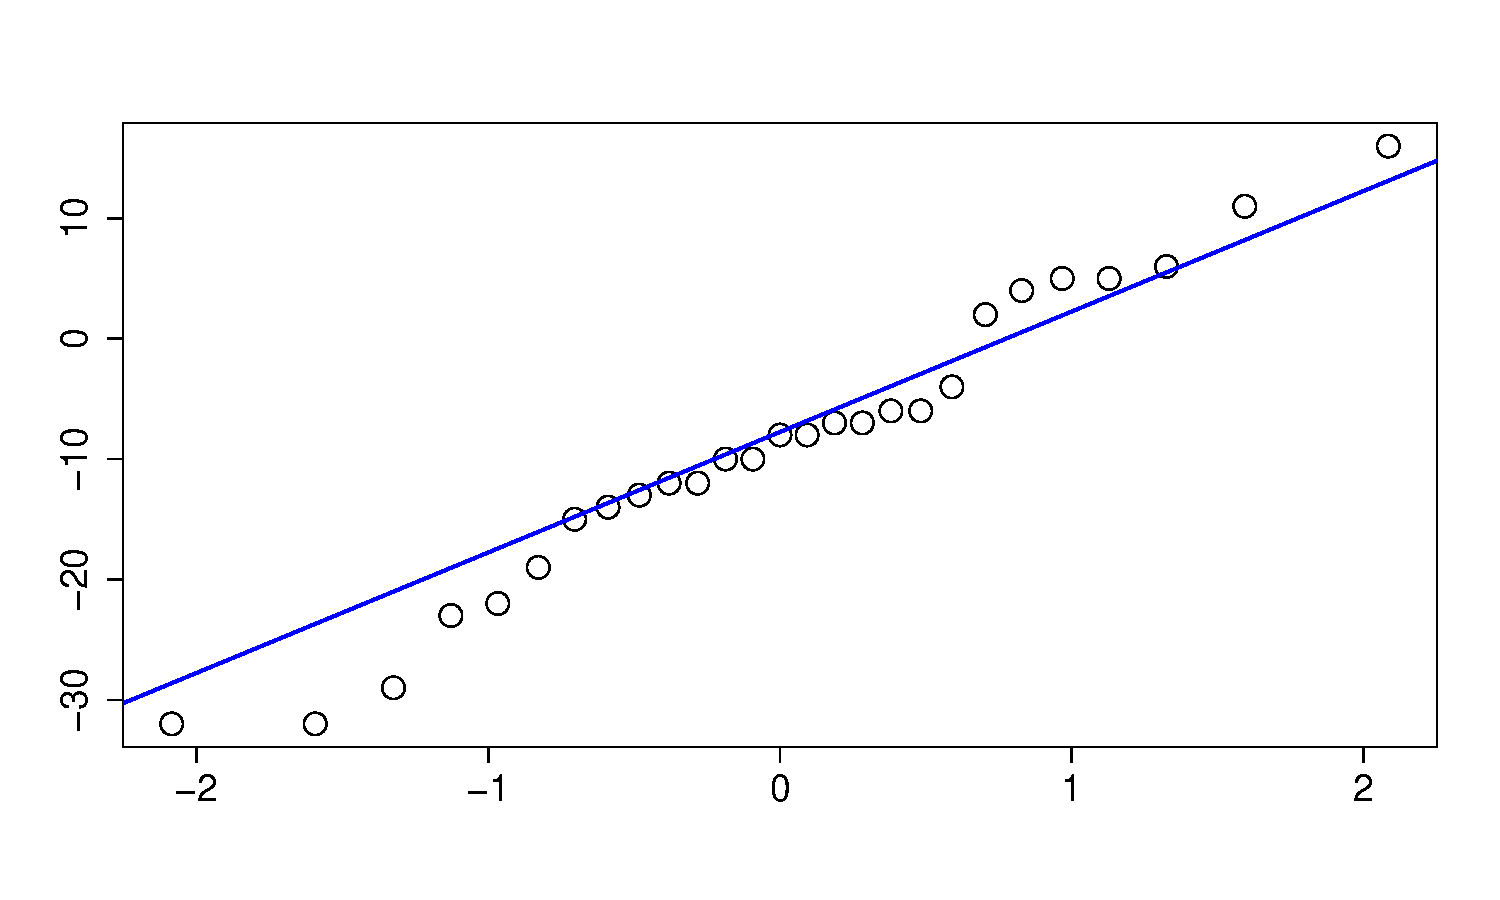
\includegraphics[width=.8\columnwidth]{experimentResults/TempoNormalidade.pdf}
%     \caption{Sample distribution related to effort.}
%     \label{fig:DistTempo}
% \end{figure}

% The sample having been tested for normality, fortunately, it was possible to perform the test of the first hypothesis established in this experiment.
Once we performed the normality tests on the sample, we carried out the hypothesis test of the average effort regarding to \textbf{RQ1.}
In the paired T-test for dependent samples, we used a significance level of $\alpha$~=~5\%, with which we reached a measure of 0.000962084 for the $p$-value.
Because it is a two-tailed test, \textit{i.e.} it includes equality in its null hypothesis, this $p$-value shows enough evidence to guarantee the rejection of the statement of $H_0: \mu Time_G = \mu Time_T$.
Therefore, we accepted the alternative hypothesis that the approaches have different efforts, once according to the test this difference is statistically significant.
% \autoref{tab:TemposGeralMedidas} shows the values enabling a dispersion analysis. 
% Whilst \autoref {fig:boxplotTempo} displays a box-plot with the variation of data observed through these data.
Figure \ref{fig:boxplotTempo} displays a box-plot with the variation of data observed through these data.
% Based on these data and their visual representation, for our surprise, it was possible to verify that, the graphical approach has an advantage over the textual approach on average.
Based on these data it was possible to verify that the graphical approach has an advantage on average.

% \begin{table}[!htb]
%     \caption{Measures related to average effort.}
%     \label{tab:TemposGeralMedidas}
%     \centering
%     \scriptsize
%     \begin{tabular}{lcc}
%     \toprule
%     \multicolumn{1}{c}{\textbf{}} &
%     \multicolumn{2}{c}{\textbf{Treatments}}
%     \\
%     \multicolumn{1}{l}{\textbf{Measures}} &
%     \multicolumn{1}{c}{\textbf{Graphical}} &
%     \multicolumn{1}{c}{\textbf{Textual}}
%     \\
%     \midrule
%         Maximum	            &	60.00   &   60.00   \\
%         3\degree~Quartile	&	28.00   &   43.00   \\
%         Median	            &	25.00   &   33.00   \\
%         Average	            &	26.37	&   35.26   \\
%         1\degree~Quartile	&	21.00	&   27.00   \\
%         Minimum         	&	12.00   &   15.00   \\
%         Standard Deviation  &  	10.12	&	14.03	\\
%     \bottomrule
%     \end{tabular}
% \end{table}

\begin{figure}[!htb]
    \centering
    % 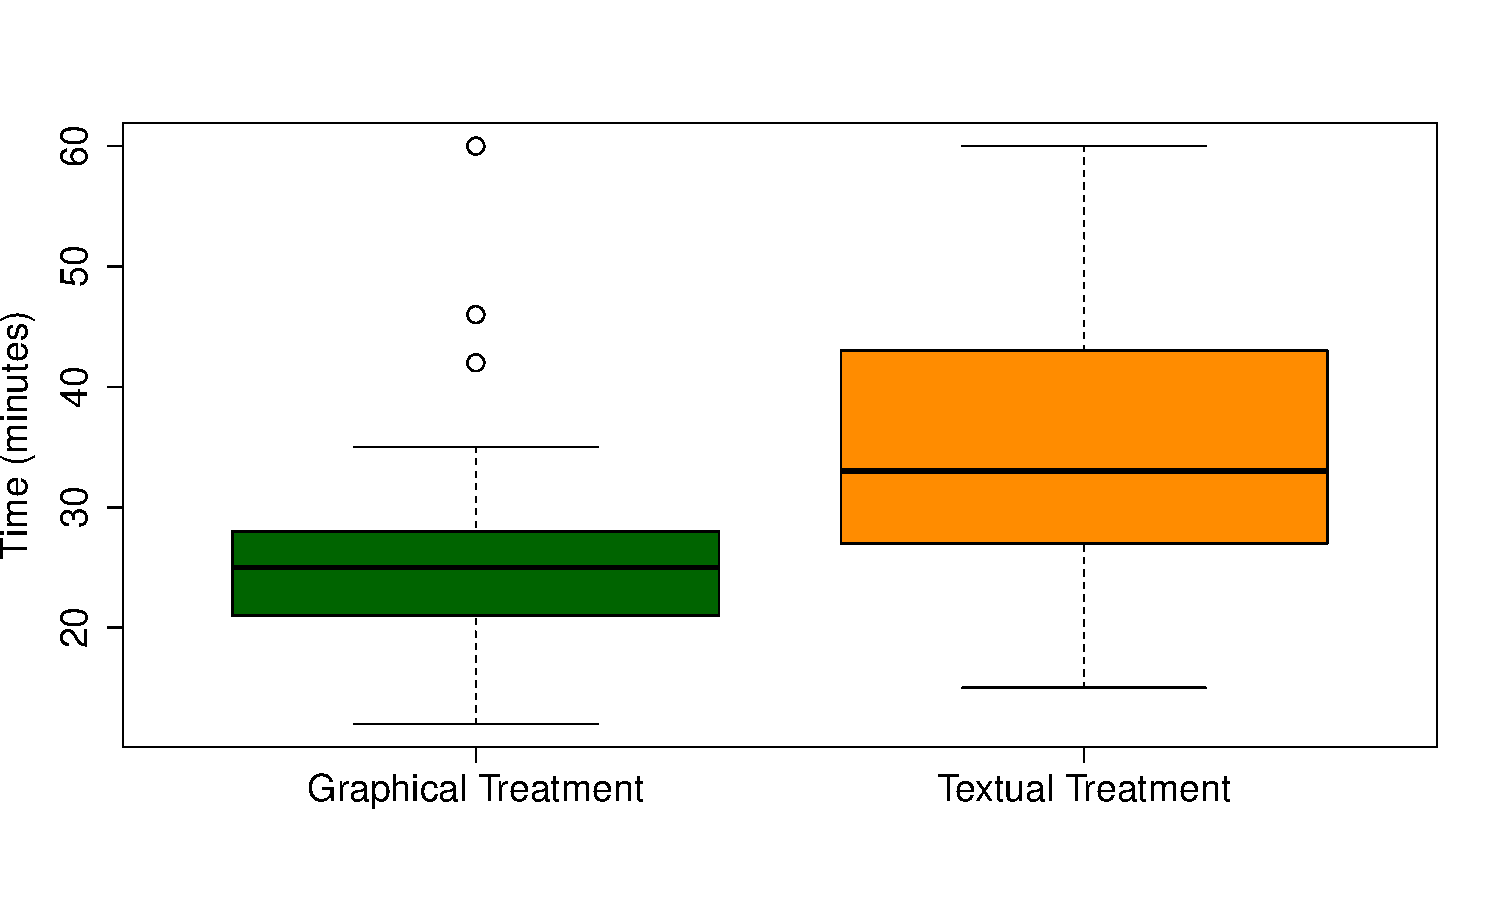
\includegraphics[width=.9\columnwidth]{experimentResults/EsforcoBoxplot.pdf}
    % \begin{tikzpicture}
%   \begin{axis}
%     [
    % boxplot/draw direction=y,
    % xtick={1, 2},
    % ylabel={\footnotesize Time (minutes)},
    % xticklabels={{\footnotesize Graphical Treatment}, {\footnotesize Textual Treatment}},
    % height= 5cm
%     ]
%     \addplot+[fill=olive, fill opacity=0.7, draw=black,
%     boxplot prepared={
%       median=25.00,
%       upper quartile=28.00,
%       lower quartile=21.00,
%       upper whisker=60.00,
%       lower whisker=12.00
%     },
%     ] coordinates {};
%     \addplot+[fill=teal, fill opacity=0.7, draw=black,
%     boxplot prepared={
%       median=33.00,
%       upper quartile=43.00,
%       lower quartile=27.00,
%       upper whisker=60.00,
%       lower whisker=15.00
%     },
%     ] coordinates {};
%   \end{axis}
% \end{tikzpicture}

\begin{filecontents*}{data.csv}
12,12,17,18,20,20,21,21,22,22,22,22,25,25,26,26,27,28,28,28,28,28,31,35,42,46,60
15,16,18,18,20,20,26,28,28,28,30,30,32,33,35,36,38,38,38,41,45,48,56,57,58,60,60
\end{filecontents*}

\begin{tikzpicture}
    \pgfplotstableread[col sep=comma]{data.csv}\csvdata
    % Boxplot groups columns, but we want rows
    \pgfplotstabletranspose\datatransposed{\csvdata} 
    \begin{axis}[
        boxplot/draw direction=y,
        xtick={1, 2},
        ylabel={\footnotesize Time (minutes)},
        xticklabels={{\footnotesize Graphical Treatment}, {\footnotesize Textual Treatment}},
        height= 4cm,
        width= 8cm,
        % boxplot/draw direction = y,
        % axis x line* = bottom,
        % axis y line = left,
        % enlarge y limits,
        ymajorgrids,
        % xtick = {1, 2},
        % xticklabel style = {align=center, font=\small},
        % xticklabels = {Graphical Treatment, Textual Treatment},
        % ylabel = {Time (minutes)},
        ytick = {15, 30, 45, 60}
    ]
        \foreach \n in {1,...,2} {
            \addplot+[boxplot, fill, fill opacity=0.4, draw=black] table[y index=\n] {\datatransposed};
        }
    \end{axis}
\end{tikzpicture}


    \caption{Box-plot - Effort per treatments.}
    \label{fig:boxplotTempo}
\end{figure}

% Vamos colocar essa planilha no Zenodo
% \begin{table*}[!htb]
%     \caption{Evaluation of the models produced in the experiment.}
%     \label{tab:ResultsModelosIndividual}
%     \centering
%     \footnotesize
%     \begin{tabular}{ccccccccccc}%{c|ccccc|ccccc}
%     \toprule
%     \multicolumn{1}{c}{} &
%     \multicolumn{5}{c}{\textbf{Graphical Treatment}} &
%     \multicolumn{5}{c}{\textbf{Textual Treatment}}
%     \\ 
%     \cmidrule{2-11}
%     \textbf{Subjects} & \textbf{MI} & \textbf{RI} & \textbf{Precision (\%)} & \textbf{Recall (\%)} & \textbf{F-measure (\%)} &
%     \textbf{MI} & \textbf{RI} & \textbf{Precision (\%)} & \textbf{Recall (\%)} & \textbf{F-Measure (\%)}
%     \\
%     \midrule
%     01	&	23	&	17	&	73.91	&	36.96	&	49.28	&	29	&	24	&	82.76	&	60.00	&	69.57	\\
%     02	&	41	&	33	&	80.49	&	84.62	&	82.50	&	67	&	41	&	61.19	&	87.23	&	71.93	\\
%     03	&	38	&	28	&	73.68	&	71.79	&	72.73	&	50	&	42	&	84.00	&	89.36	&	86.60	\\
%     04	&	36	&	25	&	69.44	&	64.10	&	66.67	&	44	&	32	&	72.73	&	68.09	&	70.33	\\
%     05	&	32	&	26	&	81.25	&	66.67	&	73.24	&	31	&	28	&	90.32	&	59.57	&	71.79	\\
%     06	&	32	&	24	&	75.00	&	61.54	&	67.61	&	38	&	36	&	94.74	&	76.60	&	84.71	\\
%     07	&	37	&	32	&	86.49	&	69.57	&	77.11	&	23	&	21	&	91.30	&	52.50	&	66.67	\\
%     08	&	41	&	34	&	82.93	&	87.18	&	85.00	&	44	&	39	&	88.64	&	97.50	&	92.86	\\
%     09	&	36	&	31	&	86.11	&	79.49	&	82.67	&	36	&	30	&	83.33	&	63.83	&	72.29	\\
%     10	&	38	&	33	&	86.84	&	84.62	&	85.71	&	20	&	19	&	95.00	&	40.43	&	56.72	\\
%     11	&	40	&	35	&	87.50	&	76.09	&	81.40	&	29	&	25	&	86.21	&	62.50	&	72.46	\\
%     12	&	53	&	33	&	62.26	&	84.62	&	71.74	&	53	&	42	&	79.25	&	89.36	&	84.00	\\
%     13	&	37	&	34	&	91.89	&	73.91	&	81.93	&	48	&	35	&	72.92	&	87.50	&	79.55	\\
%     14	&	46	&	33	&	71.74	&	84.62	&	77.65	&	36	&	29	&	80.56	&	61.70	&	69.88	\\
%     15	&	29	&	27	&	93.10	&	69.23	&	79.41	&	41	&	37	&	90.24	&	78.72	&	84.09	\\
%     16	&	33	&	25	&	75.76	&	54.35	&	63.29	&	34	&	30	&	88.24	&	75.00	&	81.08	\\
%     17	&	39	&	26	&	66.67	&	66.67	&	66.67	&	45	&	37	&	82.22	&	78.72	&	80.43	\\
%     18	&	40	&	35	&	87.50	&	89.74	&	88.61	&	45	&	43	&	95.56	&	91.49	&	93.48	\\
%     19	&	27	&	24	&	88.89	&	52.17	&	65.75	&	51	&	32	&	62.75	&	80.00	&	70.33	\\
%     20	&	25	&	24	&	96.00	&	52.17	&	67.61	&	34	&	25	&	73.53	&	62.50	&	67.57	\\
%     21	&	36	&	33	&	91.67	&	71.74	&	80.49	&	35	&	30	&	85.71	&	75.00	&	80.00	\\
%     22	&	34	&	29	&	85.29	&	74.36	&	79.45	&	44	&	38	&	86.36	&	80.85	&	83.52	\\
%     23	&	42	&	32	&	76.19	&	82.05	&	79.01	&	41	&	27	&	65.85	&	57.45	&	61.36	\\
%     24	&	28	&	19	&	67.86	&	41.30	&	51.35	&	26	&	19	&	73.08	&	47.50	&	57.58	\\
%     25	&	36	&	32	&	88.89	&	82.05	&	85.33	&	38	&	35	&	92.11	&	74.47	&	82.35	\\
%     26	&	34	&	13	&	38.24	&	33.33	&	35.62	&	31	&	18	&	58.06	&	38.30	&	46.15	\\
%     27	&	31	&	26	&	83.87	&	56.52	&	67.53	&	37	&	31	&	83.78	&	77.50	&	80.52	\\
%     \bottomrule
%     \end{tabular}
%     \begin{tablenotes}
%     \centering
%     \footnotesize
%     \item \textit{Legend: MI = Modeled Items; RI = Relevant Items.}
%     \end{tablenotes}
% \end{table*}

%#################################################################
%\subsubsection{Effectiveness}
%#################################################################

\textbf{Effectiveness}: To answer \textbf{RQ2.} regarding the effectiveness of the use of approaches, we evaluated the artifacts produced by the subjects according to the established reference models. 
% In this evaluation, we used F-Measure from the area of pattern recognition and information retrieval. 
F-Measure represents the combination of the observed accuracy and recallability of a result in relation to a reference.
By definition, this combination refers to Precision and Recall metrics, where Precision is the fraction of recovered instances that are relevant and Recall is the fraction of relevant instances that are recovered.

% After obtaining the F-Measure values for each model, we performed the Shapiro-Wilk normality test.
In addiction, we performed the Shapiro-Wilk normality test to F-Measure for each model. 
After calculations with the set of differences in F-Measure for each model, we reached a $p$-value of 0.404455.
With this test result, the chance of type 1 error (rejecting a null hypothesis that is correct) can be very high, and can be translated into 40.45\% (0.404455).
As the $p$-value > $\alpha$, we accepted the null hypothesis, thus realizing that the data is normally distributed, \textit{i.e.} the difference between the data sample and the normal distribution is not large enough to be statistically significant.
% \autoref{fig:distMedidaF} presents the visual representation of the distribution of the set of differences of the F-Measure of the models.
% \begin{figure}[!htb]
%     \centering
%     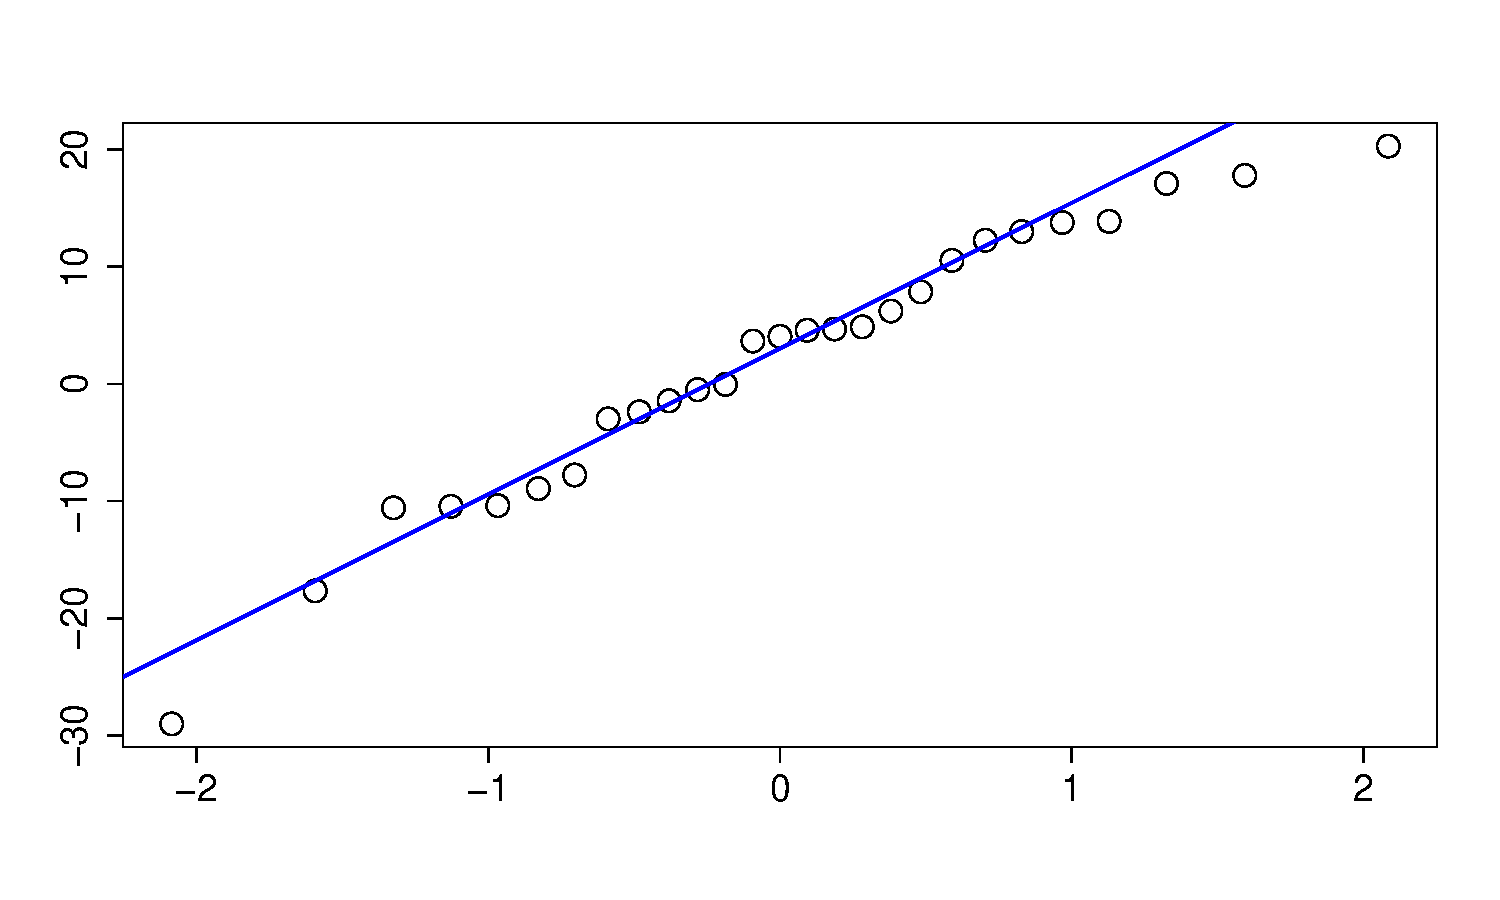
\includegraphics[width=.8\columnwidth]{experimentResults/FScoreNormalidade.pdf}
%     \caption{Sample distribution related to effectiveness.}
%     \label{fig:distMedidaF}
% \end{figure}
After the sample was tested for normality, we tested the second hypothesis defined in this experiment.
This time, in the paired sample T-test, we used again a significance level of $\alpha$~=~5\%, with which we reached a measure of 0.396468 for the $p$-value.

By the original statement including an equality, also characterizing this test as two-tailed, it was concluded that the calculated $p$-value demonstrates that there is not enough evidence to guarantee the rejection of the statement of the original null hypothesis, denoted as $ H_0: \mu Effectiveness_G = \mu Effectiveness_T$.
Therefore, we accepted the null hypothesis that the approaches have equal effectiveness, because according to the statistical test, the average difference of F-Measure between treatments is not statistically significant.
Table \ref{tab:ResultsModelosGeral} shows average measures of the evaluated values, and also provides the possibility to carry out a dispersion analysis.
\begin{table*}[!htb]
    \caption{Measures of the conceptual data models produced in the experiment.}
    \label{tab:ResultsModelosGeral}
    \centering
    \scriptsize
    \begin{tabular}{lcccccccccc}%{l|ccccc|ccccc}
    \toprule
    \multicolumn{1}{l}{} &
    \multicolumn{5}{c}{\textbf{Graphical Treatment}} &
    \multicolumn{5}{c}{\textbf{Textual Treatment}}
    \\ 
    \cmidrule{2-11}
    \textbf{Measure} & \textbf{MI} & \textbf{RI} & \textbf{Precision(\%)} & \textbf{Recall(\%)} & \textbf{F-Measure(\%)} &
    \textbf{MI} & \textbf{RI} & \textbf{Precision(\%)} & \textbf{Recall(\%)} & \textbf{F-Measure(\%)}
    \\
    \midrule
Maximum	&	53.00	&	35.00	&	96.00	&	89.74	&	88.61	&	67.00	&	43.00	&	95.56	&	97.50	&	93.48	\\
3\degree Quartile	&	39.50	&	33.00	&	87.50	&	82.05	&	81.66	&	44.50	&	37.00	&	89.44	&	80.43	&	82.93	\\
Median	&	36.00	&	29.00	&	82.93	&	71.74	&	77.11	&	38.00	&	31.00	&	83.78	&	75.00	&	72.46	\\
Average	&	35.70	&	28.26	&	79.61	&	68.57	&	72.79	&	38.89	&	31.30	&	81.50	&	70.88	&	74.73	\\
1\degree Quartile	&	32.00	&	25.00	&	73.80	&	59.03	&	67.10	&	32.50	&	26.00	&	73.30	&	60.85	&	69.72	\\
Minimum	&	23.00	&	13.00	&	38.24	&	33.33	&	35.62	&	20.00	&	18.00	&	58.06	&	38.30	&	46.15	\\
SD	&	6.33	&	5.63	&	11.94	&	15.39	&	12.16	&	9.97	&	7.30	&	10.44	&	15.36	&	10.94	\\
    \bottomrule
\end{tabular}
\begin{tablenotes}
    \footnotesize
    \centering
    \item \textit{Legend: SD = Standard Deviation; MI = Modeled Items; RI = Relevant Items.}
\end{tablenotes}
\end{table*}
Figure \ref{fig:BoxPlotMedidaF} box-plot graph displays of the F-Measure for each treatment applied. 
Based on this graph, it is possible to verify the result obtained in the hypothesis test because the data dispersion does not present much difference between the approaches.

\begin{figure}[!htb]
    \centering
    % 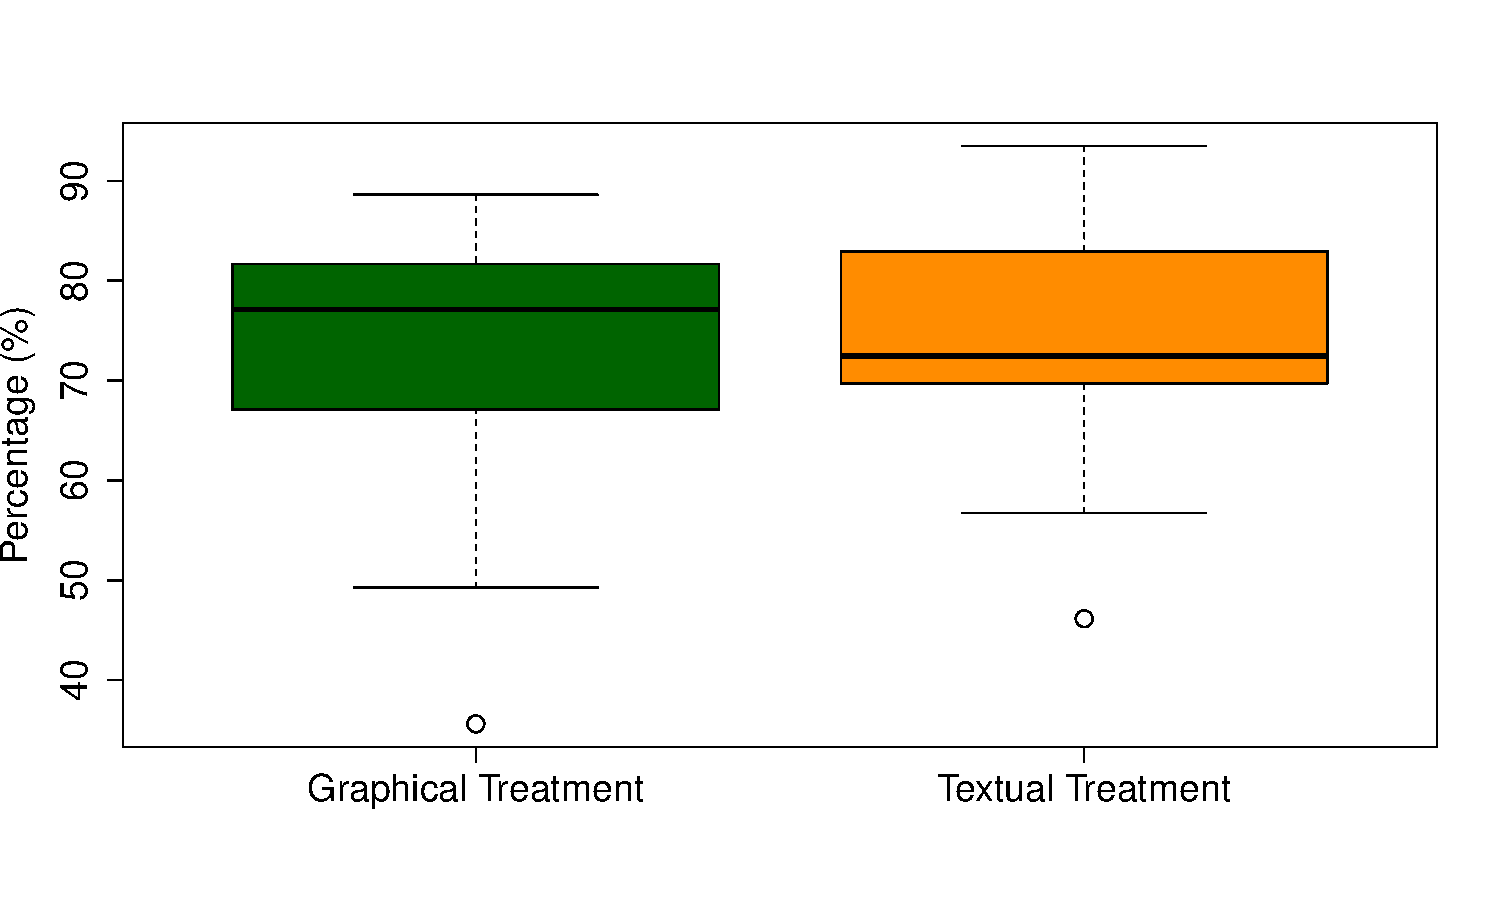
\includegraphics[width=.9\columnwidth]{experimentResults/EfetividadeBoxplot.pdf}
    % \begin{tikzpicture}
%   \begin{axis}
%     [
%     boxplot/draw direction=y,
%     xtick={1, 2},
%     ylabel={\footnotesize Percentage (\%)},
%     xticklabels={{\footnotesize Graphical Treatment}, {\footnotesize Textual Treatment}},
%     height= 5cm
%     ]
%     \addplot+[fill=olive, fill opacity=0.7, draw=black,
%     boxplot prepared={
%       median=77.11,
%       upper quartile=81.66,
%       lower quartile=67.10,
%       upper whisker=88.61,
%       lower whisker=35.62
%     },
%     ] coordinates {};
%     \addplot+[fill=teal, fill opacity=0.7, draw=black,
%     boxplot prepared={
%       median=72.46,
%       upper quartile=82.93,
%       lower quartile=69.72,
%       upper whisker=93.48,
%       lower whisker=46.15
%     },
%     ] coordinates {};
%   \end{axis}
% \end{tikzpicture}

\begin{filecontents*}{data2.csv}
35.62,49.28,51.35,63.29,65.75,66.67,66.67,67.53,67.61,67.61,71.74,72.73,73.24,77.11,77.65,79.01,79.41,79.45,80.49,81.4,81.93,82.5,82.67,85,85.33,85.71,88.61
46.15,56.72,57.58,61.36,66.67,67.57,69.57,69.88,70.33,70.33,71.79,71.93,72.29,72.46,79.55,80,80.43,80.52,81.08,82.35,83.52,84,84.09,84.71,86.6,92.86,93.48
\end{filecontents*}

\begin{tikzpicture}
    \pgfplotstableread[col sep=comma]{data2.csv}\csvdata
    % Boxplot groups columns, but we want rows
    \pgfplotstabletranspose\datatransposed{\csvdata} 
    \begin{axis}[
         boxplot/draw direction=y,
        xtick={1, 2},
        ylabel={\footnotesize Percentage (\%)},
        xticklabels={{\footnotesize Graphical Treatment}, {\footnotesize Textual Treatment}},
        height= 4cm,
        width= 8cm,
        % boxplot/draw direction = y,
        % axis x line* = bottom,
        % axis y line = left,
        % enlarge y limits,
        ymajorgrids,
        % xtick = {1, 2},
        % xticklabel style = {align=center, font=\small},
        % xticklabels = {Graphical Treatment, Textual Treatment},
        % ylabel = {Percentage (\%)},
        ytick = {25, 40, 60, 80, 100}
    ]
        \foreach \n in {1,...,2} {
            \addplot+[boxplot, fill, fill opacity=0.4, draw=black] table[y index=\n] {\datatransposed};
        }
    \end{axis}
\end{tikzpicture}
    \caption{Box-plot - F-Measure per treatments.}
    \label{fig:BoxPlotMedidaF}
\end{figure}

%#################################################################
%\subsubsection{Qualitative Evaluation}
%#################################################################

\textbf{Qualitative Evaluation}: took place with the analysis of the two instruments applied after the modeling tasks.
The first was used to respond to \textbf{RQ3.} regarding the Perceived Ease Of Use (PEOU) and Perceived Usefulness (PU) of treatments, according to the TAM model \citep{Davis:1989}. 
%\citep{Persico:2014}.
This occurred through the selection of quality attributes described in ISO/IEC 25010.
For this, we established a Likert scale from one to six points.
This scale served to measure the level of agreement of the subjects in the face of the statements exposed in the form.
We chosen an even number of alternatives to avoid possible neutral responses.
Thus, the seven quality attributes are grouped in three categories, being defined as follows:

\begin{inparadesc}
    \item \textbf{Functionality}: 
        \begin{inparadesc}
            \item \textit{Conformity}: ability level to which the software to achieve specified goals with  functional completeness, correctness and appropriateness related to their functionalities.
        \end{inparadesc}
   
    \item \textbf{Usability}: 
        \begin{inparadesc}
            %Appropriateness recognisability
            \item \textit{Understandability}: ability level to which users can recognize whether a software is appropriate for their needs; 
            \item \textit{Learnability}: ability level to which the software enables the user to learn how to use it with effectiveness, efficiency in emergency situations;
            \item \textit{Operability}: ability level to which the software is easy to operate, control and appropriate to use.
        \end{inparadesc}
    
    \item \textbf{Quality in Use}: 
        \begin{inparadesc}
            \item \textit{Quality in Use}: ability level to which the software to achieve specified goals with effectiveness and efficiency with their users in specific contexts of use;
            % Performance Efficiency
            \item \textit{Productivity}: ability level to which the software to achieve specified goals with time-behavior, resources utilization and capacity, when performing its functions, meet requirements;
            \item \textit{Satisfaction}: ability level to which the software to achieve specified goals with usefulness, trust, pleasure and comfort with their users in specific contexts of use.
        \end{inparadesc}
\end{inparadesc}

After summarizing the results, we observed a good acceptance by the subjects for the ERtext tool, developed in this work.
Figure \ref{fig:inst3GERALExp} synthesizes the responses received for each quality attributes, showing a certain degree of similarity in the subjects perception during the treatments application.
A point that can be emphasized is the set of positive responses in relation to the Productivity quality attribute, since in the hypothesis test related to the effort, the treatment using the brModelo demonstrated a lesser need for execution time.

In analyzing the open comments on this evaluation form, which asked subjects to indicate positive and negative points of the tools, it was explicitly reported that the code completion feature provided a sense of agility in the modeling database process.

\begin{figure}[!htb]
    \centering
    % 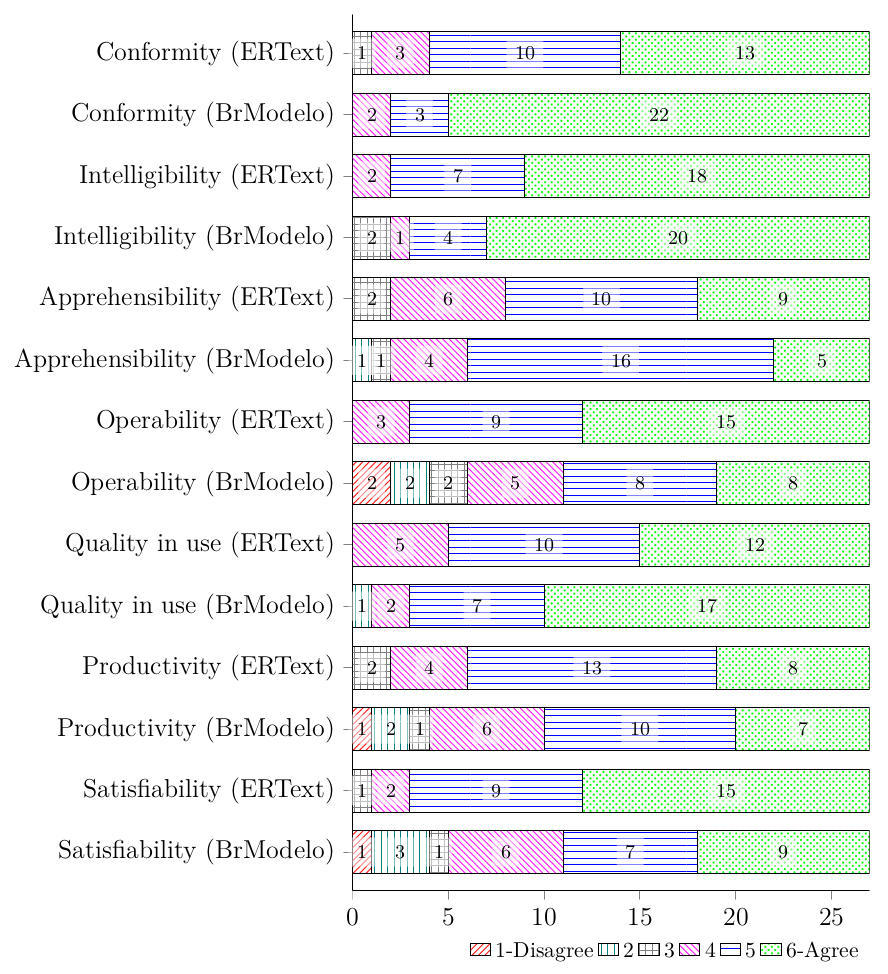
\includegraphics[width=.9\columnwidth]{experimentResults/Inst3.png}
    \pgfplotsset{testbar/.style={
        xbar stacked,
        legend cell align=left,
        legend style={
            legend columns=6,
            font=\scriptsize,
            at={(xticklabel cs:1.0)},
            anchor=north east,
            draw=none
            },
        width=5.75cm,
        axis y line*= none, 
        axis x line*= bottom,
        xmajorgrids = false,
        xmin=0,xmax=27,
        ytick = data,
        yticklabels = {
            {\scriptsize Conformity-ERtext},
            {\scriptsize Conformity-brModelo},
            {\scriptsize Understandability-ERtext}, %Intelligibility
            {\scriptsize Understandability-brModelo},
            {\scriptsize Learnability-ERtext}, %Apprehensibility
            {\scriptsize Learnability-brModelo}, 
            {\scriptsize Operability-ERtext},
            {\scriptsize Operability-brModelo},
            {\scriptsize Quality in Use-ERtext},
            {\scriptsize Quality in Use-brModelo},
            {\scriptsize Productivity-ERtext}, %Performance Efficiency
            {\scriptsize Productivity-brModelo},
            {\scriptsize Satisfaction-ERtext},
            {\scriptsize Satisfaction-brModelo}
        },
        tick align = outside, xtick pos = left,
        bar width=3.2mm, y=6.3mm,
        y=4.4mm,
        enlarge y limits={abs=0.450},% 0.5 + 0.5*(y - bar width)/y [TeX.sx #47995]
        nodes near coords,
        nodes near coords align=center,%Move values in bar
        every node near coord/.append style={
            black,
            font=\scriptsize,
            text opacity=1,
            fill=white,
            fill opacity=0.5,
            outer sep=\pgflinewidth
        }
    }}
    \begin{tikzpicture}
    \begin{axis}[testbar] 
    \addplot[pattern color=red,pattern=north east lines] coordinates
        {(0,14)(0,13)(0,12)(0,11)(0,10)(0,9)(0,8)(2,7)(0,6)(0,5)(0,4)(1,3)(0,2)(1,1)};
    \addplot[pattern color=teal,pattern=vertical lines] coordinates
        {(0,14)(0,13)(0,12)(0,11)(0,10)(1,9)(0,8)(2,7)(0,6)(1,5)(0,4)(2,3)(0,2)(3,1)};
    \addplot[pattern color=gray, pattern=grid] coordinates
       {(1,14)(0,13)(0,12)(2,11)(2,10)(1,9)(0,8)(2,7)(0,6)(0,5)(2,4)(1,3)(1,2)(1,1)};
    \addplot[pattern color=magenta, pattern=north west lines] coordinates
       {(3,14)(2,13)(2,12)(1,11)(6,10)(4,9)(3,8)(5,7)(5,6)(2,5)(4,4)(6,3)(2,2)(6,1)};
    \addplot[pattern color=blue, pattern=horizontal lines] coordinates
       {(10,14)(3,13)(7,12)(4,11)(10,10)(16,9)(9,8)(8,7)(10,6)(7,5)(13,4)(10,3)(9,2)(7,1)};
    \addplot[pattern color=green, pattern=crosshatch dots] coordinates
       {(13,14)(22,13)(18,12)(20,11)(9,10)(5,9)(15,8)(8,7)(12,6)(17,5)(8,4)(7,3)(15,2)(9,1)};
    \legend{1-Disagree, 2, 3, 4, 5, 6-Agree}
    \end{axis}
    \end{tikzpicture}
    
% \begin{tikzpicture}
% \begin{axis}[
%     xbar stacked,
%     legend cell align=center,
%     legend style={
%     legend columns=5,
%         at={(xticklabel cs:1.0)},
%         anchor=north east,
%         draw=none
%     },
%     ytick=data,
%     axis y line*=none,
%     axis x line*=bottom,
%     tick label style={font=\small},
%     legend style={font=\small},
%     label style={font=\small},
%     xtick={0,3,6},
%     xticklabel= {},
%     bar width=5mm,
%     ylabel={Questions},
%     yticklabels={P-Q1, T-Q1, P-Q2, T-Q2, P-Q3, T-Q3, P-Q4, T-Q4,P-Q5, T-Q5,P-Q6, T-Q6, P-Q7, T-Q7},
%     xmin=0,
%     xmax=6,
%     area legend,
%     y=6.5mm,
%     enlarge y limits={abs=0.625},
%     nodes near coords,
%     nodes near coords align=center,
%     every node near coord/.append style={
%         black,
%         font=\small,
%         text opacity=.65,
%         fill=white,
%         fill opacity=0.75,
%         outer sep=\pgflinewidth
%     }
% ]
% \addplot[pattern color=red,pattern=horizontal lines] coordinates
% {(0,14)(0,13)(0,12)(0,11) (3,10)(0,9)(0,8) (0,7) (0,6)(0,5)(0,4) (0,3) (0,2) (0,1)};   
% \addplot[pattern color=orange,pattern=grid] coordinates
% {(3,14) (0,13)(0,12)(0,11)(2,10) (1,9)(1,8)(0,7)(3,6)(0,5)(0,4)(3,3) (4,2) (0,1) };  
% \addplot[pattern color = green, pattern=crosshatch dots] coordinates
% {(0,14) (0,13) (3,12)(2,11)(1,10) (3,9)(4,8)(1,7)(3,6)(1,5)(3,4)(2,3)(2,2) (2,1) };   
% \addplot[pattern color=blue, pattern =vertical lines ] coordinates
% {(2,14) (3,13) (2,12)(3,11)(0,10)(2,9)(1,8)(4,7)(0,6)(3,5) (3,4)(1,3)(0,2)(4,1)};   
% \addplot[pattern color=gray, pattern = dots] coordinates
% {(1,14)(3,13)(1,12)(1,11)(0,10)(0,9)(0,8)(1,7) (0,6)(2,5) (0,4)(0,3)(0,2)(0,1) };   
% \legend{1-Disagree, 2, 3, 4, 5-Agree}

% \end{axis}
% \end{tikzpicture}
% \footnotesize
% T-Thoth answers; P-Parsifal answers;






% \begin{tikzpicture}
% \begin{axis}[
%     xbar stacked,
%     legend cell align=left,
%     legend style={
%     legend columns=2,
%         at={(xticklabel cs:1.0)},
%         anchor=north east,
%         draw=none
%     },
%     ytick=data,
%     axis y line*=none,
%     axis x line*=bottom,
%     tick label style={font=\scriptsize},
%     legend style={font=\scriptsize},
%     %legend style={font=\scriptsize,row sep=-0.1cm,/tikz/every odd column/.append style={column sep=0.01cm}},
%     label style={font=\scriptsize},
%     xtick={0,10,...,100},
%     width=\columnwidth,
%     bar width=3.5mm,
%     % xlabel={Frequencia em \%},
%     yticklabels={
%     {Q1 - OC},
%     {Q2 - TD},
%     {Q3 - OC},
%     {Q4 - TD},
%     {Q5 - OC},
%     {Q6 - TD},
%     {Q7 - OC},
%     {Q8 - TD},
%     {Q9 - OC},
%     {Q10 - TD},
%     {Q11 - OC},
%     {Q12 - TD}},
%     xmin=0,
%     xmax=100,
%     area legend,
%     y=5mm,
%     enlarge y limits={abs=0.625},
%     nodes near coords,
%     nodes near coords={\pgfmathprintnumber\pgfplotspointmeta\%},
%     nodes near coords align=center,%Move values in bar
%     every node near coord/.append style={
%         black,
%         font=\footnotesize,
%         text opacity=1,
%         fill=white,
%         fill opacity=0.7,
%         outer sep=\pgflinewidth
%     }
% ]
% \addplot[pattern color=blue,pattern=dots] coordinates
% {(0,0)(0,1)(0,2)(0,3)(0,4)(0,5)(0,6)(0,7)(0,8)(0,9)(0,10)(0,11)};
% \addplot[pattern color=red, pattern=vertical lines] coordinates
% {(4,0)(32,1)(0,2)(9,3)(13,4)(18,5)(0,6)(9,7)(5,8)(5,9)(0,10)(14,11)};
% \addplot[pattern color=cyan, pattern=grid] coordinates
% {(27,0)(9,1)(4,2)(5,3)(23,4)(27,5)(36,6)(23,7)(27,8)(41,9)(46,10)(45,11)};
% \addplot[pattern color=green, pattern=horizontal lines] coordinates
% {(55,0)(32,1)(55,2)(68,3)(41,4)(50,5)(46,6)(64,7)(64,8)(45,9)(36,10)(27,11)};
% \addplot[pattern color=orange, pattern=crosshatch dots] coordinates
% {(14,0)(27,1)(41,2)(18,3)(23,4)(5,5)(18,6)(4,7)(4,8)(9,9)(18,10)(14,11)};
% \legend{Strongly disagree,Disagree,Neither agree nor disagree,Agree,Strongly agree}; 

% \end{axis}  
% \end{tikzpicture}d
    \caption{Quality attributes per treatments.}
    \label{fig:inst3GERALExp}
\end{figure}

\begin{figure}[!htb]
    \centering
    % 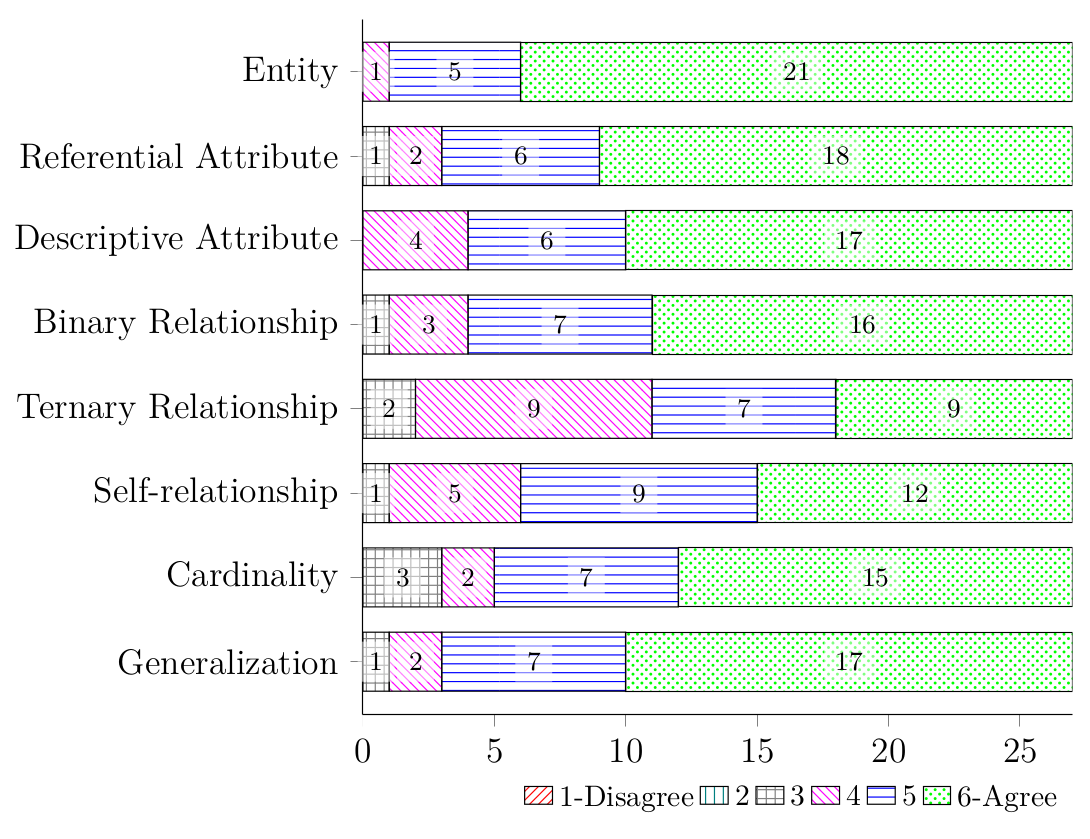
\includegraphics[width=0.9\columnwidth]{experimentResults/Inst4.png}
    \pgfplotsset{testbar/.style={
            xbar stacked,
            legend cell align=left,
            legend style={
                legend columns=6,
                font=\footnotesize,
                at={(xticklabel cs:1.0)},
                anchor=north east,
                draw=none
                },
            width=6.6cm,
            axis y line*= none, 
            axis x line*= bottom,
            xmajorgrids = false,
            xmin=0,xmax=27,
            ytick = data,
            yticklabels = {
            {\scriptsize Entity}, 
            {\scriptsize Referential Attribute},
            {\scriptsize Descriptive Attribute},
            {\scriptsize Binary Relationship},
            {\scriptsize Ternary Relationship}, 
            {\scriptsize Self-relationship},
            {\scriptsize Cardinality},
            {\scriptsize Generalization}
            },
            tick align = outside, xtick pos = left,
             bar width=3.2mm, y=6.3mm,
             y=4.4mm,
             enlarge y limits={abs=0.450},% 0.5 + 0.5*(y - bar width)/y [TeX.sx #47995] #47995]
            nodes near coords,
            nodes near coords align=center,%Move values in bar
            every node near coord/.append style={
                black,
                font=\scriptsize,
                text opacity=1,
                fill=white,
                fill opacity=0.5,
                outer sep=\pgflinewidth
            }
        }}
    \begin{tikzpicture}
    \begin{axis}[testbar] 
    \addplot[pattern color=red,pattern=north east lines] coordinates
        {(0,8) (0,7) (0,6) (0,5) (0,4) (0,3) (0,2) (0,1)};
    \addplot[pattern color=teal,pattern=vertical lines] coordinates
        {(0,8) (0,7) (0,6) (0,5) (0,4) (0,3) (0,2) (0,1)};   
    \addplot[pattern color=gray, pattern=grid] coordinates
        {(0,8) (1,7) (0,6) (1,5) (2,4) (1,3) (3,2) (1,1)};   
    \addplot[pattern color=magenta, pattern=north west lines] coordinates
        {(1,8) (2,7) (4,6) (3,5) (9,4) (5,3) (2,2) (2,1)};   
    \addplot[pattern color=blue, pattern=horizontal lines] coordinates
        {(5,8) (6,7) (6,6) (7,5) (7,4) (9,3) (7,2) (7,1)};   
    \addplot[pattern color=green, pattern=crosshatch dots] coordinates
        {(21,8) (18,7) (17,6) (16,5) (9,4) (12,3) (15,2) (17,1)};  
    \legend{1-Disagree, 2, 3, 4, 5, 6-Agree}
    \end{axis}
    \end{tikzpicture}

% \begin{figure}[!ht]
% \centering
% \caption{Resultados do formulários de avaliação.}
% \begin{tikzpicture}
% \begin{axis}[
%     xbar stacked,
%     legend cell align=center,
%     legend style={
%     legend columns=5,
%         at={(xticklabel cs:1.0)},
%         anchor=north east,
%         draw=none
%     },
%     ytick=data,
%     axis y line*=none,
%     axis x line*=bottom,
%     tick label style={font=\small},
%     legend style={font=\small},
%     label style={font=\small},
%     xtick={0,5,10},
%     xticklabel= {},
%     bar width=7mm,
%     ylabel={Formulário/Grupo},
%     yticklabels={F1-C, F1-E, F2-C, F2-E, F3-C, F3-E},
%     xmin=0,
%     xmax=10,
%     area legend,
%     y=9mm,
%     enlarge y limits={abs=0.825},
%     nodes near coords,
%     nodes near coords align=center,
%     every node near coord/.append style={
%         black,
%         font=\small,
%         text opacity=.65,
%         fill=white,
%         fill opacity=0.6,
%         outer sep=\pgflinewidth
%     }
% ]
% %NOTA 1
% \addplot[pattern color=red,pattern=horizontal lines] coordinates
% {(0,6)(0,5)(0,4)(0,3)(0,2)(0,1)};
% %NOTA 2
% \addplot[pattern color=orange,pattern=grid] coordinates
% {(1,6)(1,5)(1,4)(0,3)(1,2)(0,1)};   
% \addplot[pattern color = green, pattern=crosshatch dots] coordinates
% % NOTA 3
% {(3,6)(3,5)(5,4)(2,3)(5,2)(1,1)};   
% \addplot[pattern color=blue, pattern =vertical lines ] coordinates
% %NOTA 4
% {(2,6)(3,5)(1,4)(4,3)(3,2)(3,1)};   
% \addplot[pattern color=gray, pattern = dots] coordinates
% %NOTA 5
% {(3,6)(3,5)(2,4)(4,3)(0,2)(6,1)};   
% \legend{1-Disagree, 2, 3, 4, 5-Agree}

% \end{axis}
% \end{tikzpicture}
% \footnotesize
% \label{img:respostas1}
% 	\fonte{O autor.}
% \end{figure}
    \caption{Evaluation of DSL designers.}
    \label{fig:inst4GERALExp}
\end{figure}

With regard to \textbf{RQ4.} on the assessment of DSL designers, we analyzed the artifacts of the 2nd qualitative assessment instrument.
This instrument listed the 8 ER modeling builders covered by DSL, arranged with a Likert scale from one to six points.
Again, an even number was chosen on the scale to avoid neutral responses that could lead to a more subjective bias.

Figure \ref{fig:inst4GERALExp} compiles all the responses received, the builders related to Entities and Descriptive Attributes were the best evaluated, with all 27 agreeing with their current representation.
In contrast, all the other 6 obtained at least one disagreement.
In this sense, the contributors of Ternary Relationship and Cardinality stand out, with 2 and 3 evaluations disagreeing with their current representations respectively.

%#######################################################
%#######################################################
\section{\uppercase{Threats to validity}}
\label{sec:threats}
%#######################################################%#######################################################

% In empirical studies it is necessary to analyze and discuss the threats to validity, as well as the strategies used to mitigate them.
% For the list of possible threats, we adopted the classification scheme published by Cook and Campbell \cite{Cook:1979}, which is divided in four types of threats.
% These threats followed the proposed pattern and were divided into four categories, namely: construct validity, internal validity, external validity and conclusion validity.

In this section we discuss the main threats to validity of our study and present the strategies we used to mitigate them~\citep{Cook:1979}.
%We follow the strategies of~\citet{Cook:1979}.

\textbf{Construct Validity} - 
% The construct validity concerns the experiment design and social factors.
\textit{Inappropriate Pre-operational Explanation}:
% This threat is related to the fact that the experiment did not have the objective of the artifacts sufficiently defined before translation into measures or treatments.
To mitigate this threat, the effort of each approach was compared, as well as their effectiveness carried out according to the Precision and Recall metrics. 
% of F-Measure.
\textit{Interaction of Different Treatments}: 
% If the subjects involved in one more study, the controls of the different studies, can change and reverberate in the final results.
%As this experiment 
We followed a paired design, all subjects are executed both treatments.
However, learning issues among the execution of activities were not observed.
This can be verified through the analyzed distributions normality of the both samples: effort and effectiveness, demonstrating that the results remained similar as a whole with a low variation, \textit{i.e.} low standard deviation indicates that the data points tend to be very close to the mean.
% This can be selected through the distributions normality analyzed of the effort and effectiveness samples, as which demonstrate that  results had kept similar as a whole.
% \textit{Hypothesis Prediction}: 
% % When subjects participate in an experiment it is possible that they try to find out what the objective or intended experiment result is.
% This threat can bias the behavior, positively or negatively, depending on the anticipated hypothesis.
% To mitigate this threat, we not informed the subjects about further details of the experiment.
% , \textit{e.g.} research questions, hypotheses, objectives and purpose.

\textbf{Internal Validity} - 
% Threats to internal validity are influences that can affect independent variables in correlation to causality, without the researcher's knowledge.
\textit{History}:
% There is a risk when a specific time period influences the experiment performance. 
To soothe this threat, we carried out the experiment in an academic environment, and because we conducted the entire process in August, when in general students are not necessarily overwhelmed with academic activities.
%, \textit{e.g.} tests and assignments.
\textit{Maturation}:
% This is the threat that occurs in relation to the subjects reacting in different ways over time.
% Examples are when subjects are affected negatively (tiredness or boredom) or positively (learning) during the experiment execution.
In order to alleviate this threat, we informed subjects from the beginning that they could terminate their participation at any time, without any penalty.
% \textit{Tests}:
% If the tests are repeated, the subjects may respond differently at different times, as they know how the test is performed.
% If there is a need to familiarize yourself with the tests, it is important that the test results are not returned to the subject, so as not to support unintentional learning.
% There was no need for repetition of activities, since they were performed once per participant in each treatment.
%\textit{Instrumentation}:
% This threat is related to the artifacts used to perform the experiment, such as data collection forms, etc.
% If these are poorly designed, the experience is negatively affected.
% To combat this threat, all artifacts were previously checked and validated at meetings between the researchers involved in this work.
% In addition, we carried out a pilot study to validate the protocol planned for the experiment.

\textbf{External Validity} - 
% Threats to external validity are conditions related to experiment replication.
\textit{Experiment Subjects}:
% The subjects selected for the experiment may not include a significant group for an study area.
Seeking to mitigate this threat, the experiment was carried out with undergrad students of Software Engineering and Computer Science programs, and soon, inserted in the context of using the conceptual modeling of relational databases.
However, the fact that the sample has less than 30 subjects is a statistical threat in the analyzed area, and it was not possible to mitigate this fact.
\textit{Subjects Interaction with the Evaluation Artifacts}:
% This is the threat related to the application of the experiment evaluation artifacts with the subjects.
Depending on the moment this can affect the experimental results.
For instance, if a questionnaire is answered a few days after the execution experiment, people tend to answer differently than they would do moments after the activities.
% \textit{Configuration and Treatment Interaction}:
% % They are threats related to the use of an unrepresentative configuration or material.
% To soften this threat, documentation was used based on templates and traditional models found in database teaching material.
% In addition, the artifacts were validated with two specialists in the field of SE.
%Software Engineering.
% An important point regarding external validity is that threats can be reduced by making the experimental environment as realistic as possible.
% On the other hand, reality is not always homogeneous.
%However, more important is to define and report the characteristics of the environment, such as the team's experience, tools, assessment methods and applicability in a specific context \cite{Wohlin:2012}.

\textbf{Conclusion Validity} - 
\textit{Low Statistical Power}:
To try mitigating this threat, some statistical methods were adopted, such as the Shapiro-Wilk normality test, the paired T-test as a hypothesis test for dependent samples, and the F-Measure for qualitative analysis of the models produced.
\textit{Reliability of Measurements}:
% The reliability of the measurements used has a direct impact on the validity of the experiment as a whole. 
To mitigate this threat, it was adopted objective measurements that did not depend on subjective judgment (effort, measured in time spent, and F-Measure).
On the other hand, the metrics used for the qualitative evaluation still served as a complementary input in the discussion of the results obtained.
\textit{Experimental Environment}:
% The experiment must be carried out in a controlled environment, avoiding external influences.
In order to mitigate this possible threat, we instructed subjects that conversations could not take place during the entire activities execution, or leave the environment or access electronic devices.

%#######################################################
%#######################################################
\section{\uppercase{Conclusion}}
\label{sec:conclusion}
%#######################################################%#######################################################

%With the results obtained it was possible to answer the four RQs of the experiment, as well as the two associated hypotheses.
This study presented a controlled experiment evaluating ERText, a proposed textual DSL for database conceptual modeling. ERText is compared with the brModelo, a graphical DSL well-known in Software Engineering ER lectures. 
% In this sense, three quality attributes from these DSLs are analyzed: representation effort, representation effectiveness and productivity. 

From the analysis it is possible to highlight the following aspects:
\begin{inparaenum}[(i)]
\item Effort: the graphical approach to ER modeling requires less effort to perform the evaluated tasks. However, we considered that this difference is small and it can be reduced with future improvements in the proposed DSL.
\item Effectiveness: the computed average difference states that there is no differences between the approaches, \textit{i.e.}, one approach is not better than the other. 
However, we observed that there is a need to carry out tests involving problems of greater complexities for better assessment.
\item Qualitative comparison between treatments: We observed a certain balance between treatments, but with a positive evaluation for ERtext regarding the 
%quality attribute 
``Productivity'' attribute.
Because it was the first time that the subjects had contact with our grammar, and also considering a first release of our DSL, we conclude that ERText is on the rails for achieving better productivity indexes.
\end{inparaenum}

%\textbf{Evaluation of the proposed language}:
We also collected qualitative feedback from participants. 
As a result, there are some improvements regarding the language design that need to be revised, in particular to the cardinalities and ternary relationships.
% Since the continuity of language development is foreseen, the execution of a possible refactoring, and also the implementation of new ER builders, is a natural step for its software evolution.
From the experimental results we conclude that there is feasibility and good perspectives for the motivated context, i.e., as a  tool for teaching entity-relationship modeling with the differential of adopting a textual approach for conceptual database modeling in classrooms instead of a graphical notation. 
% This is sustained by the results, which did not obtained expressive differences with regard to the evaluated quality attributes from ERText in comparison to a mature graphical DSL. 
This conclusion is sustained by the results, which did not obtained expressive differences with regard to the evaluated quality attributes between the tools.
% Hence, we conclude that ERText, as a textual DSL, is a good alternative for those that dislike graphical representations of database models, opening doors for complementary classroom strategies in teaching database conceptual modeling.  

\section*{\uppercase{Acknowledgements}}
\noindent This study was partially funded by PROPESQ through AGP, and by FAPERGS, through the ARD project N\textsuperscript{\underline{o}}19/2551-0001268-3.


\bibliographystyle{apalike}
{\small
\bibliography{ICEIS-Bib}}


% \section*{\uppercase{Appendix}}

% \noindent If any, the appendix should appear directly after the references without numbering, and not on a new page. To do so please use the following command:
% \textit{$\backslash$section*\{APPENDIX\}}

\end{document}

